% !TeX program = xelatex
% 第二十二章 各种积分间的联系与场论初步
\chapter{各种积分间的联系与场论初步}

本章给出联系二重积分与曲线积分、三重积分与曲面积分、空间曲面积分与曲线积分的重要公式，分别称为格林（G.\ Green，$1793$—$1841$）公式，高斯公式以及斯托克斯（G.\ Stokes，$1819$—$1903$）公式．它们可以看作牛顿－莱布尼茨公式的高维推广．场论是多元函数微积分学最重要应用的部分．本章还将给出上述三个公式在场论中的解释．本章的内容是为学习数学物理与近代分析准备必要的基础．

\section{各种积分间的联系}

\subsection{格林公式}

在讲这个公式以前，先介绍平面单连通区域的概念．

一个平面区域 $D$，如果全落在此区域内的任何一条封闭曲线都可以不经过 $D$ 以外的点而连续地收缩为属于 $D$ 的一点，则称 $D$ 为平面单连通区域．否则称为复连通区域．例如上半平面 $y\geqslant 0$ 是平面单连通区域，$x^{2}+y^{2}\leqslant 1$ 也是平面单连通区域，而 $x^{2}+y^{2}\geqslant 1$ 和 $0<x^{2}+y^{2}<1$ 都是复连通区域．可见，单连通区域就是不含有``洞''甚至``点洞''的区域（图~\ref{fig:22-1}），而复连通区域就是含有``洞''的区域（图~\ref{fig:22-2}）．

\begin{figure}[htbp]
\centering
\begin{minipage}[c]{0.42\textwidth}\centering
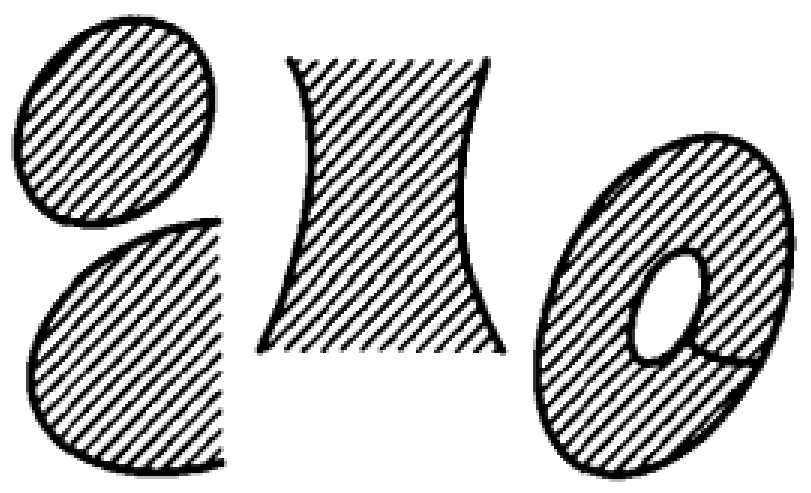
\includegraphics[width=\textwidth]{work/figures/fig22-1}\caption{\relax}\label{fig:22-1}
\end{minipage}\hfill
\begin{minipage}[c]{0.42\textwidth}\centering
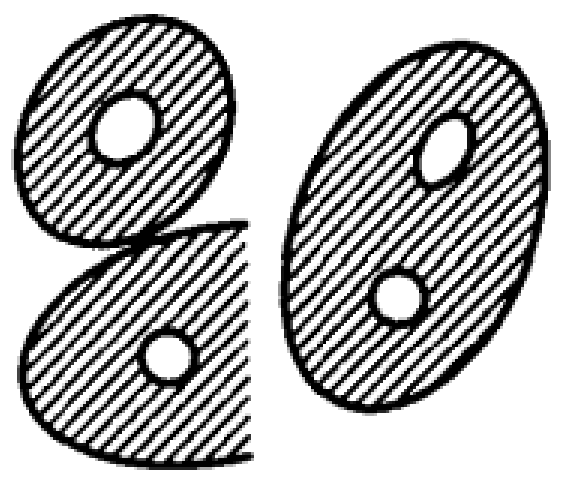
\includegraphics[width=\textwidth]{work/figures/fig22-2}\caption{\relax}\label{fig:22-2}
\end{minipage}
\end{figure}

\begin{theorem}[格林公式]\label{thm:22-1}
设 $D$ 是由逐段光滑闭曲线 $L$ 围成的平面单连通闭区域，函数 $P(x,y)$，$Q(x,y)$ 在 $D$ 上有一阶连续偏导数，则有
\begin{equation}\label{eq:green}
\iint_{D}\left(\frac{\partial Q}{\partial x}-\frac{\partial P}{\partial y}\right)\mathrm{d}x\mathrm{d}y=\oint_{L}P\mathrm{d}x+Q\mathrm{d}y, \tag{1}
\end{equation}
其中右端的积分路径是闭曲线 $L$，方向取正向．
\end{theorem}

回忆闭曲线正向的含义是，当一人沿曲线 $L$ 正向行走时，曲线 $L$ 所包围的区域 $D$ 恒在人的左边．

\begin{proof}
（1）先考虑区域是最简单的情形．设 $D$ 既可表为
\[
D=\left\{(x,y)\mid y_{1}(x)\leqslant y\leqslant y_{2}(x),\,a\leqslant x\leqslant b\right\},
\]
又可表为
\[
D=\left\{(x,y)\mid x_{1}(y)\leqslant x\leqslant x_{2}(y),\,c\leqslant y\leqslant d\right\}.
\]
即从上下来看，$D$ 由 $y=y_{2}(x)$ 与 $y=y_{1}(x)$（$a\leqslant x\leqslant b$）围成，而从左右来看，$D$ 是由 $x=x_{2}(y)$ 和 $x=x_{1}(y)$（$c\leqslant y\leqslant d$）围成（见图~\ref{fig:22-3}）．这时用牛顿－莱布尼茨公式和第二型曲线积分与定积分的关系，有
\begin{figure}[htbp]
\centering
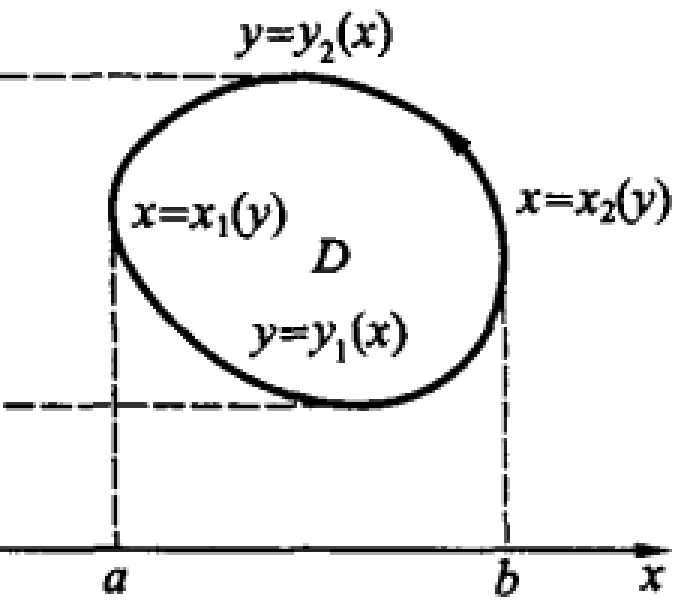
\includegraphics[width=0.30\textwidth]{work/figures/fig22-3}\caption{\relax}\label{fig:22-3}
\end{figure}
\[
\begin{aligned}
\iint_{D}\frac{\partial Q}{\partial x}\mathrm{d}x\mathrm{d}y&=\int_{c}^{d}\mathrm{d}y\int_{x_{1}(y)}^{x_{2}(y)}\frac{\partial Q}{\partial x}\mathrm{d}x\\
&=\int_{c}^{d}\left[Q\left(x_{2}(y),y\right)-Q\left(x_{1}(y),y\right)\right]\mathrm{d}y\\
&=\int_{L_{1}}Q(x,y)\mathrm{d}y+\int_{L_{2}}Q(x,y)\mathrm{d}y\\
&=\oint_{L}Q(x,y)\mathrm{d}y.
\end{aligned}
\]
其中 $\displaystyle\int_{L_{1}}$ 与 $\displaystyle\int_{L_{2}}$ 分别表示沿右边的曲线 $x=x_{2}(y)$ 与左边的曲线 $x=x_{1}(y)$ 按 $L$ 的方向的第二型曲线积分．同理
\[
\begin{aligned}
\iint_{D}\frac{\partial P}{\partial y}\mathrm{d}x\mathrm{d}y&=\int_{a}^{b}\mathrm{d}x\int_{y_{1}(x)}^{y_{2}(x)}\frac{\partial P}{\partial y}\mathrm{d}y\\
&=\int_{a}^{b}\left[P\left(x,y_{2}(x)\right)-P\left(x,y_{1}(x)\right)\right]\mathrm{d}x\\
&=-\oint_{L}P(x,y)\mathrm{d}x.
\end{aligned}
\]
因此
\[
\iint_{D}\left(\frac{\partial Q}{\partial x}-\frac{\partial P}{\partial y}\right)\mathrm{d}x\mathrm{d}y=\oint_{L}P(x,y)\mathrm{d}x+Q(x,y)\mathrm{d}y.
\]
（2）如果区域如图~\ref{fig:22-4}，则公式\eqref{eq:green}仍然成立．事实上，这时\eqref{eq:green}的证明对 $\displaystyle\iint_{D}\frac{\partial Q}{\partial x}\mathrm{d}x\mathrm{d}y$
\begin{figure}[htbp]
\centering
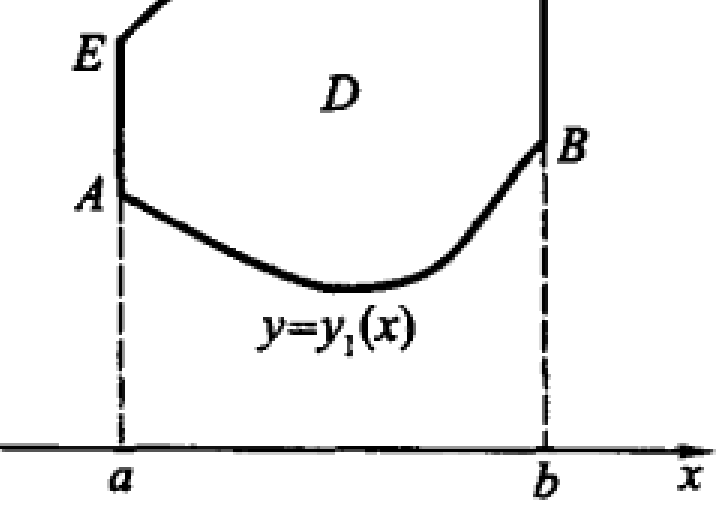
\includegraphics[width=0.30\textwidth]{work/figures/fig22-4}\caption{\relax}\label{fig:22-4}
\end{figure}
完全适用．对另一项的证明需稍作修改．
\[
\begin{aligned}
\iint_{D}\frac{\partial P}{\partial y}\mathrm{d}x\mathrm{d}y&=\int_{a}^{b}\mathrm{d}x\int_{y_{1}(x)}^{y_{2}(x)}\frac{\partial P}{\partial y}\mathrm{d}y\\
&=\int_{a}^{b}\left[P\left(x,y_{2}(x)\right)-P\left(x,y_{1}(x)\right)\right]\mathrm{d}x\\
&=-\left[\int_{\widehat{AB}}P(x,y)\mathrm{d}x+\int_{\widehat{CE}}P(x,y)\mathrm{d}x\right].
\end{aligned}
\]
注意到 $\widehat{BC}$ 与 $\widehat{EA}$ 是两条平行于 $y$ 轴的直线，根据第二型曲线积分的定义，必然有
\[
\int_{\widehat{BC}}P(x,y)\mathrm{d}x=\int_{\widehat{EA}}P(x,y)\mathrm{d}x=0.
\]
把它们加到上面等式的右边，便得
\[
\begin{aligned}
\iint_{D}\frac{\partial P}{\partial y}\mathrm{d}x\mathrm{d}y&=-\left(\int_{\widehat{AB}}P\,\mathrm{d}x+\int_{\widehat{BC}}P\,\mathrm{d}x+\int_{\widehat{CE}}P\,\mathrm{d}x+\int_{\widehat{EA}}P\,\mathrm{d}x\right)\\
&=-\oint_{L}P(x,y)\mathrm{d}x,
\end{aligned}
\]
这样便证明了公式\eqref{eq:green}成立．

同理，对如图~\ref{fig:22-5} 的区域 $D$，公式也是成立的．
\begin{figure}[htbp]
\centering
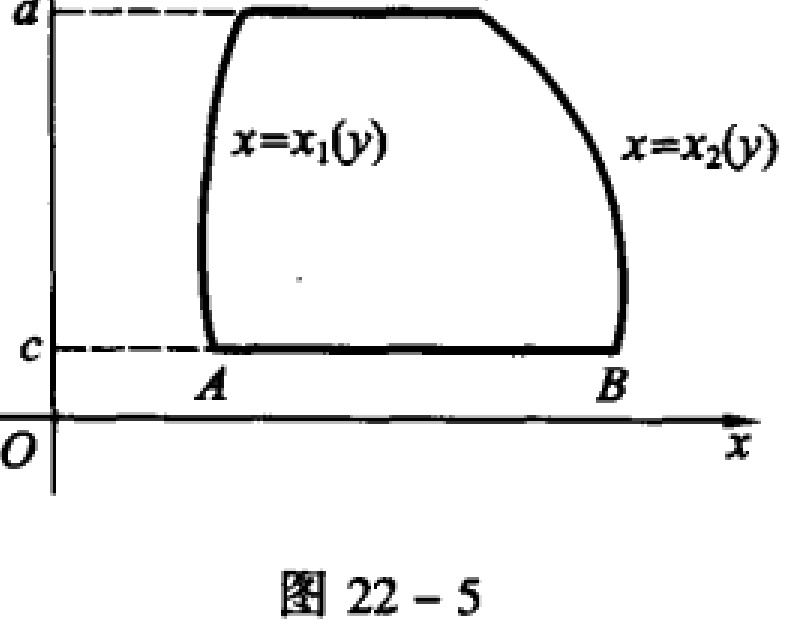
\includegraphics[width=0.30\textwidth]{work/figures/fig22-5}\caption{\relax}\label{fig:22-5}
\end{figure}

（3）如果区域可用若干条光滑曲线分成有限个（1）或（2）中讨论过的区域，则公式仍然成立．事实上，例如图~\ref{fig:22-6}，用直线段 $AB$ 把 $D$ 分成三个（2）讨论过的区域 $D_{1}$、$D_{2}$ 和 $D_{3}$．利用（2）中已证的结果，有
\begin{figure}[htbp]
\centering
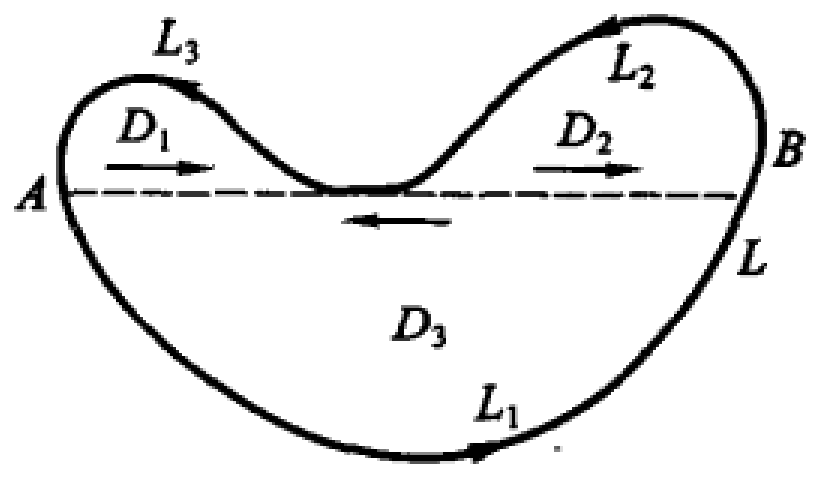
\includegraphics[width=0.30\textwidth]{work/figures/fig22-6}\caption{\relax}\label{fig:22-6}
\end{figure}
\[
\begin{aligned}
\iint_{D}\left(\frac{\partial Q}{\partial x}-\frac{\partial P}{\partial y}\right)\mathrm{d}x\mathrm{d}y&=\sum_{i=1}^{3}\iint_{D_{i}}\left(\frac{\partial Q}{\partial x}-\frac{\partial P}{\partial y}\right)\mathrm{d}x\mathrm{d}y\\
&=\sum_{i=1}^{3}\int_{L_{i}}P\mathrm{d}x+Q\mathrm{d}y\\
&=\oint_{L}P\mathrm{d}x+Q\mathrm{d}y,
\end{aligned}
\]
最后一个等式成立是因为沿直线 $AB$ 的两个不同方向各积分了一次，因此相应项积分的和为零．定理~\ref{thm:22-1} 证完．
\end{proof}

其实，对复连通区域，公式也是成立的，如图~\ref{fig:22-7}，我们用两条直线段 $AB$ 与 $CE$ 把复连通区域 $D$ 分成两个前面讨论过的区域 $D_{1}$、$D_{2}$，分别对 $D_{1}$、$D_{2}$ 用公式，便得到
\begin{figure}[htbp]
\centering
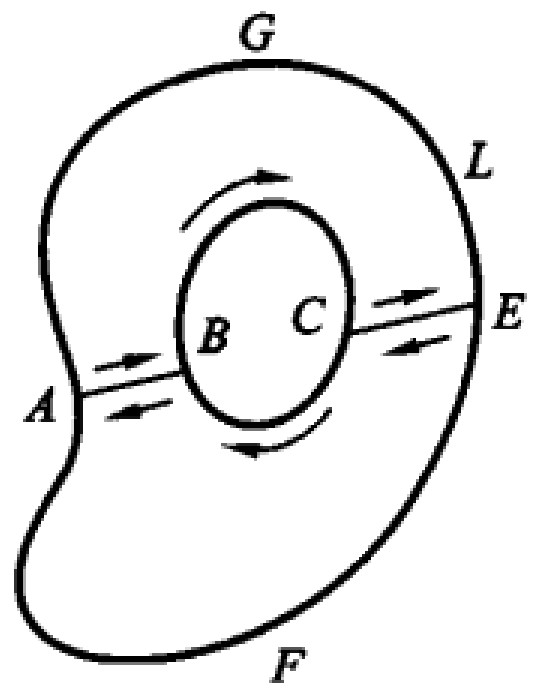
\includegraphics[width=0.22\textwidth]{work/figures/fig22-7}\caption{\relax}\label{fig:22-7}
\end{figure}
\[
\begin{aligned}
\iint_{D}\left(\frac{\partial Q}{\partial x}-\frac{\partial P}{\partial y}\right)\mathrm{d}x\mathrm{d}y&=\left(\iint_{D_{1}}+\iint_{D_{2}}\right)\left(\frac{\partial Q}{\partial x}-\frac{\partial P}{\partial y}\right)\mathrm{d}x\mathrm{d}y\\
&=\left(\int_{\widehat{ABCEGA}}+\int_{\widehat{AFECBA}}\right)P\mathrm{d}x+Q\mathrm{d}y\\
&=\oint_{L}P\mathrm{d}x+Q\mathrm{d}y,
\end{aligned}
\]
其中 $L$ 分别表示在两条闭曲线上的积分：一条沿外面的曲线按逆时针方向，一条沿内部的曲线按顺时针方向，加起来正是沿 $D$ 的全部边界 $L$ 作线积分，方向取正向：当人沿 $L$ 走时，区域 $D$ 永远在人的左边．而在推导过程中，沿 $\widehat{AB}$，$\widehat{CE}$ 的积分也是按不同方向各积分了一次，因此其和抵消而在最终结果中不出现．

对多于一个``洞''的复连通区域可类似处理．

为了便于记忆，格林公式可以写成如下的形式：
\[
\iint_{D}\begin{vmatrix}\dfrac{\partial}{\partial x}&\dfrac{\partial}{\partial y}\\[4pt] P&Q\end{vmatrix}\mathrm{d}x\mathrm{d}y=\oint_{L}P\mathrm{d}x+Q\mathrm{d}y.
\]
牛顿－莱布尼茨公式的一种解释是，它建立了函数在一个区间的定积分与其原函数在区间边界（两个点）的值之间的联系．格林公式给出了二元函数在平面区域的重积分与其``原函数''在区域边界的第二型曲线积分间的联系．从这个意义上说，格林公式可以看作牛顿－莱布尼茨公式的二维推广．

可以应用格林公式计算某些曲线积分．

\begin{example}\label{ex:22-1-1}
求 $\displaystyle\int_{\widehat{AMO}}\left(\mathrm{e}^{x}\sin y-my\right)\mathrm{d}x+\left(\mathrm{e}^{x}\cos y-m\right)\mathrm{d}y$，其中 $\widehat{AMO}$ 为由 $A(a,0)$ 至 $O(0,0)$，经上半圆周 $x^{2}+y^{2}=ax$ 的道路（图~\ref{fig:22-8}）．
\end{example}

\begin{proof}[解]
$\widehat{AMO}$ 不是封闭曲线，如果加上直线段 $\widehat{OA}$ 则构成封闭曲线 $L$．注意到沿 $\widehat{OA}$，函数 $\mathrm{e}^{x}\sin y-my$ 为 $0$，且 $\widehat{OA}$ 在 $y$ 轴上的投影为一点，因此
\[
\int_{\widehat{OA}}\left(\mathrm{e}^{x}\sin y-my\right)\mathrm{d}x+\left(\mathrm{e}^{x}\cos y-m\right)\mathrm{d}y=0.
\]
\begin{figure}[htbp]
\centering
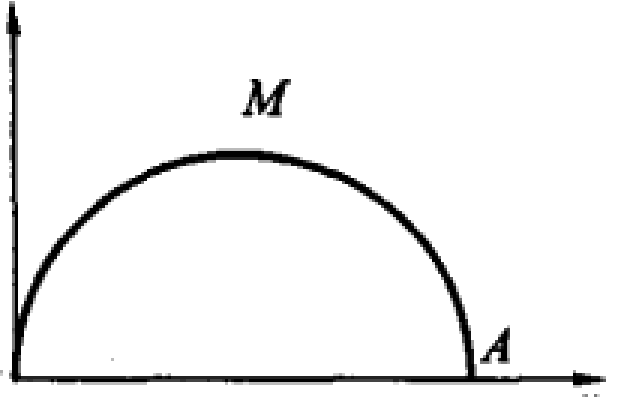
\includegraphics[width=0.26\textwidth]{work/figures/fig22-8}\caption{\relax}\label{fig:22-8}
\end{figure}
故添上 $\widehat{OA}$ 后用格林公式得
\[
\begin{aligned}
&\int_{\widehat{AMO}}\left(\mathrm{e}^{x}\sin y-my\right)\mathrm{d}x+\left(\mathrm{e}^{x}\cos y-m\right)\mathrm{d}y\\
=&\oint_{L}\left(\mathrm{e}^{x}\sin y-my\right)\mathrm{d}x+\left(\mathrm{e}^{x}\cos y-m\right)\mathrm{d}y\\
=&\iint_{D}\left(\mathrm{e}^{x}\cos y-\mathrm{e}^{x}\cos y+m\right)\mathrm{d}x\mathrm{d}y\\
=&m\iint_{D}\mathrm{d}x\mathrm{d}y=m\cdot\frac{1}{2}\pi\left(\frac{a}{2}\right)^{2}=\frac{m}{8}\pi a^{2}.
\end{aligned}
\]
\end{proof}

\begin{example}\label{ex:22-1-2}
计算 $I=\displaystyle\oint_{L}\frac{x\mathrm{d}y-y\mathrm{d}x}{x^{2}+y^{2}}$，其中 $L$ 为 $x^{2}+y^{2}=a^{2}$ 的正向．
\end{example}

\begin{proof}[解]
在 $L$ 上有 $x^{2}+y^{2}=a^{2}$，故有
\[
I=\frac{1}{a^{2}}\oint_{L}x\mathrm{d}y-y\mathrm{d}x.
\]
取 $P(x,y)=-y$，$Q(x,y)=x$，由格林公式得
\[
I=\frac{1}{a^{2}}\iint_{D}2\mathrm{d}x\mathrm{d}y=\frac{2}{a^{2}}\pi a^{2}=2\pi.
\]
\end{proof}

请读者思考，可否对 $P(x,y)=\dfrac{-y}{x^{2}+y^{2}}$，$Q(x,y)=\dfrac{x}{x^{2}+y^{2}}$ 直接用格林公式．为什么？

在例~\ref{ex:22-1-2} 中我们还看到平面区域 $D$ 的面积可以用第二型曲线积分表示为
\[
|D|=\iint_{D}\mathrm{d}x\mathrm{d}y=\frac{1}{2}\oint_{L}x\mathrm{d}y-y\mathrm{d}x.
\]
这是我们在本教程上册第八章 §2 推导过、在第二十章 §3 重积分变量代换中应用过的公式．

\begin{example}\label{ex:22-1-3}
求星形线 $x=a\cos^{3}t$，$y=b\sin^{3}t$（$0\leqslant t\leqslant 2\pi$）所围区域的面积．
\end{example}

\begin{proof}[解]
\[
\begin{aligned}
|D|&=\frac{1}{2}\oint_{L}x\mathrm{d}y-y\mathrm{d}x\\
&=\frac{1}{2}\int_{0}^{2\pi}\left[a\cos^{3}t\cdot 3b\sin^{2}t\cos t+b\sin^{3}t\cdot 3a\cos^{2}t\sin t\right]\mathrm{d}t\\
&=\frac{3}{2}ab\int_{0}^{2\pi}\sin^{2}t\cos^{2}t\,\mathrm{d}t=6ab\int_{0}^{\frac{\pi}{2}}\left(\sin^{2}t-\sin^{4}t\right)\mathrm{d}t\\
&=6ab\left(\frac{1}{2}-\frac{3\cdot 1}{4\cdot 2}\right)\frac{\pi}{2}=\frac{3}{8}\pi ab.
\end{aligned}
\]
\end{proof}

\subsection{高斯公式}

\begin{theorem}[高斯公式]\label{thm:22-2}
设空间区域 $V$ 由分片光滑的双侧封闭曲面 $S$ 围成，函数 $P(x,y,z)$，$Q(x,y,z)$，$R(x,y,z)$ 在 $V$ 及 $S$ 上有一阶连续偏导数，则有
\[
\iiint_{V}\left(\frac{\partial P}{\partial x}+\frac{\partial Q}{\partial y}+\frac{\partial R}{\partial z}\right)\mathrm{d}x\mathrm{d}y\mathrm{d}z=\oiint_{S}P\mathrm{d}y\mathrm{d}z+Q\mathrm{d}z\mathrm{d}x+R\mathrm{d}x\mathrm{d}y,
\]
其中 $S$ 的方向为外侧．
\end{theorem}

\begin{proof}
仿照格林公式的证明，先对简单的区域证明高斯公式．考虑
\[
\iiint_{V}\frac{\partial R}{\partial z}\mathrm{d}x\mathrm{d}y\mathrm{d}z=\oiint_{S}R\mathrm{d}x\mathrm{d}y,
\]
其中 $V$ 如图~\ref{fig:22-9}，它的边界由下、上、中三部分 $S_{1}$、$S_{2}$、$S_{3}$ 构成．上部为 $S_{2}$，由方程 $z=z_{2}(x,y)$ 给出，下部为 $S_{1}$，由方程 $z=z_{1}(x,y)$ 给出，中间由母线平行于 $z$ 轴的柱面 $S_{3}$ 构成．$S_{1}$ 与 $S_{2}$ 在 $Oxy$ 平面上有公共投影 $D$．$V$ 可表为
\[
V=\{(x,y,z)\mid z_{1}(x,y)\leqslant z\leqslant z_{2}(x,y),(x,y)\in D\}.
\]
$V$ 的边界曲面 $S$ 的外侧可表为
\[
\begin{aligned}
S_{1}:&\ z=z_{1}(x,y),(x,y)\in D,\ \text{下侧},\\
S_{2}:&\ z=z_{2}(x,y),(x,y)\in D,\ \text{上侧},\\
S_{3}:&\ \text{以}\ D\ \text{的边界为准线夹在}\ S_{1}\ \text{与}\ S_{2}\ \text{之间的柱面外侧}.
\end{aligned}
\]
\begin{figure}[htbp]
\centering
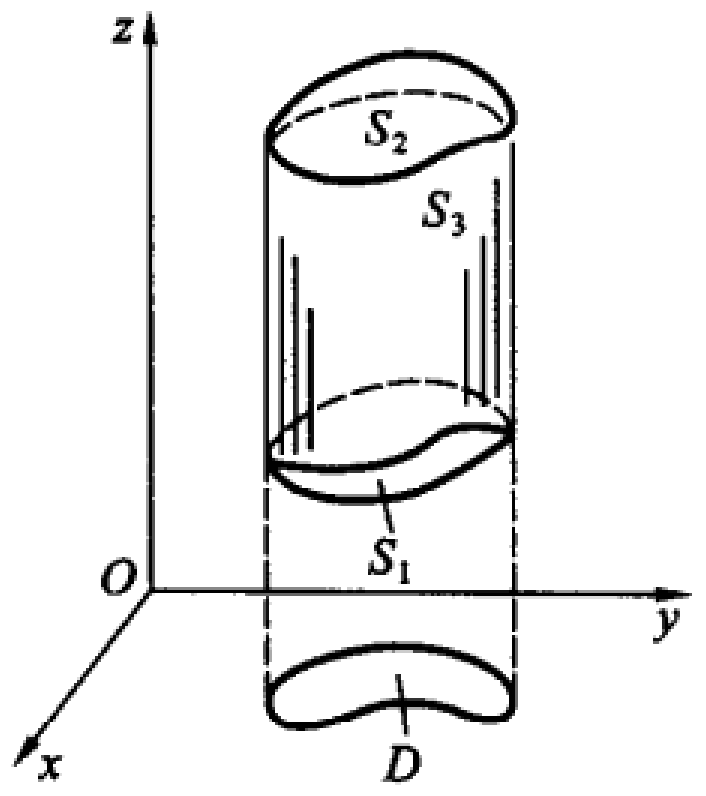
\includegraphics[width=0.28\textwidth]{work/figures/fig22-9}\caption{\relax}\label{fig:22-9}
\end{figure}
由三重积分的计算方法及第二型曲面积分的计算方法得
\[
\begin{aligned}
\iiint_{V}\frac{\partial R}{\partial z}\mathrm{d}x\mathrm{d}y\mathrm{d}z&=\iint_{D}\mathrm{d}x\mathrm{d}y\int_{z_{1}(x,y)}^{z_{2}(x,y)}\frac{\partial R}{\partial z}\mathrm{d}z\\
&=\iint_{D_{xy}}\left[R\left(x,y,z_{2}(x,y)\right)-R\left(x,y,z_{1}(x,y)\right)\right]\mathrm{d}x\mathrm{d}y\\
&=\iint_{S_{2}}R(x,y,z)\mathrm{d}x\mathrm{d}y+\iint_{S_{1}}R(x,y,z)\mathrm{d}x\mathrm{d}y\\
&=\left(\iint_{S_{1}}+\iint_{S_{2}}+\iint_{S_{3}}\right)R(x,y,z)\mathrm{d}x\mathrm{d}y\\
&=\oiint_{S}R(x,y,z)\mathrm{d}x\mathrm{d}y.
\end{aligned}
\]
上面第四个等式成立是因为 $S_{3}$ 在 $Oxy$ 面上的投影面积为零，所以
\[
\iint_{S_{3}}R(x,y,z)\mathrm{d}x\mathrm{d}y=0.
\]
同理可证
\[
\iiint_{V}\frac{\partial P}{\partial x}\mathrm{d}x\mathrm{d}y\mathrm{d}z=\oiint_{S}P\mathrm{d}y\mathrm{d}z,\qquad
\iiint_{V}\frac{\partial Q}{\partial y}\mathrm{d}x\mathrm{d}y\mathrm{d}z=\oiint_{S}Q\mathrm{d}z\mathrm{d}x.
\]
对于一般的区域 $V$，可以通过添加有限块光滑曲面，把它分为有限个上面已证明过的简单子区域的并．例如对图~\ref{fig:22-10} 和图~\ref{fig:22-11} 中的区域，高斯公式仍成立．完全类似于格林公式的推导，对每个子区域分别用高斯公式然后相加，注意到在添加的曲面上，恰好对不同的两侧各积分了一次，因而互相抵消，从而在曲面积分中不出现这些添加的曲面．定理~\ref{thm:22-2} 证完．
\end{proof}

\begin{figure}[htbp]
\centering
\begin{minipage}[c]{0.42\textwidth}\centering
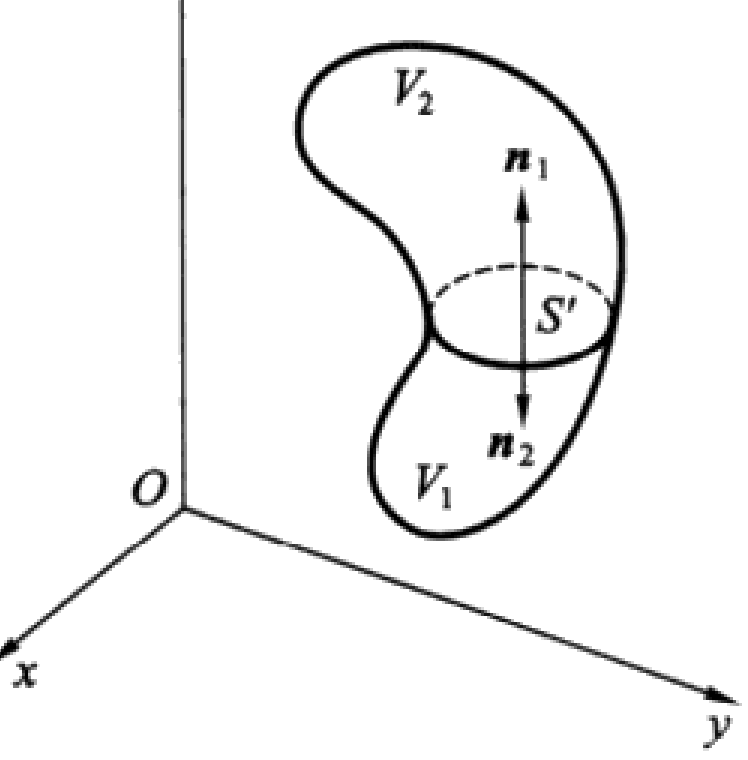
\includegraphics[width=\textwidth]{work/figures/fig22-10}\caption{\relax}\label{fig:22-10}
\end{minipage}\hfill
\begin{minipage}[c]{0.42\textwidth}\centering
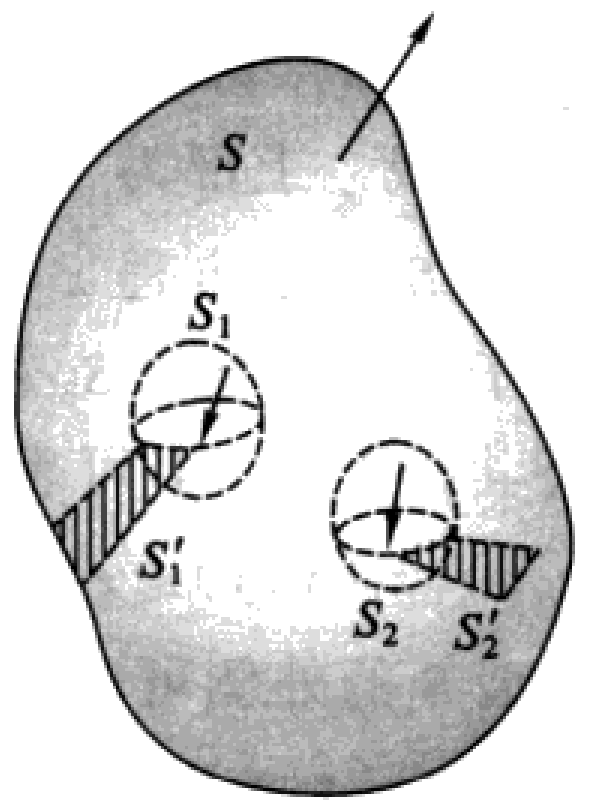
\includegraphics[width=\textwidth]{work/figures/fig22-11}\caption{\relax}\label{fig:22-11}
\end{minipage}
\end{figure}

利用两种曲面积分之间的关系，不难得到高斯公式的另一种形式
\[
\iiint_{V}\left(\frac{\partial P}{\partial x}+\frac{\partial Q}{\partial y}+\frac{\partial R}{\partial z}\right)\mathrm{d}x\mathrm{d}y\mathrm{d}z=\oiint_{S}\left(P\cos\alpha+Q\cos\beta+R\cos\gamma\right)\mathrm{d}S,
\]
其中 $\bm{n}=(\cos\alpha,\cos\beta,\cos\gamma)$ 是 $S$ 指向 $V$ 的外部的单位法向量．

高斯公式给出了函数在三维区域上的重积分与其``原函数''在区域边界上的第二型曲面积分间的联系，在这个意义上说，高斯公式是牛顿－莱布尼茨公式的三维推广．

\begin{example}\label{ex:22-1-4}
计算 $I=\displaystyle\oiint_{S}\frac{1}{x^{2}+y^{2}+z^{2}}\left(x^{3}\mathrm{d}y\mathrm{d}z+y^{3}\mathrm{d}z\mathrm{d}x+z^{3}\mathrm{d}x\mathrm{d}y\right)$，其中 $S$ 是 $x^{2}+y^{2}+z^{2}=a^{2}$ 的外侧．
\end{example}

\begin{proof}[解]
因为在 $S$ 上有 $x^{2}+y^{2}+z^{2}=a^{2}$，故
\[
I=\frac{1}{a^{2}}\oiint_{S}x^{3}\mathrm{d}y\mathrm{d}z+y^{3}\mathrm{d}z\mathrm{d}x+z^{3}\mathrm{d}x\mathrm{d}y.
\]
由高斯公式
\[
\begin{aligned}
I&=\frac{3}{a^{2}}\iiint_{V}\left(x^{2}+y^{2}+z^{2}\right)\mathrm{d}x\mathrm{d}y\mathrm{d}z\\
&=\frac{3}{a^{2}}\int_{0}^{2\pi}\mathrm{d}\theta\int_{0}^{\pi}\mathrm{d}\varphi\int_{0}^{a}r^{4}\sin\varphi\,\mathrm{d}r\\
&=\frac{12}{5}\pi a^{3}.
\end{aligned}
\]
\end{proof}

请读者思考，可否对 $P=\dfrac{x^{3}}{x^{2}+y^{2}+z^{2}}$，$Q=\dfrac{y^{3}}{x^{2}+y^{2}+z^{2}}$，$R=\dfrac{z^{3}}{x^{2}+y^{2}+z^{2}}$ 直接用高斯公式．另一个问题是为什么
\[
\iiint_{V}\left(x^{2}+y^{2}+z^{2}\right)\mathrm{d}x\mathrm{d}y\mathrm{d}z\neq a^{2}\iiint_{V}\mathrm{d}x\mathrm{d}y\mathrm{d}z.
\]

\subsection{斯托克斯公式}

\begin{theorem}[斯托克斯公式]\label{thm:22-3}
若光滑曲面 $S$ 的边界为光滑曲线 $L$，函数 $P$、$Q$、$R$ 在曲面 $S$ 及曲线 $L$ 上具有连续的一阶偏导数，则
\[
\begin{aligned}
&\iint_{S}\left(\frac{\partial R}{\partial y}-\frac{\partial Q}{\partial z}\right)\mathrm{d}y\mathrm{d}z+\left(\frac{\partial P}{\partial z}-\frac{\partial R}{\partial x}\right)\mathrm{d}z\mathrm{d}x+\left(\frac{\partial Q}{\partial x}-\frac{\partial P}{\partial y}\right)\mathrm{d}x\mathrm{d}y\\
&=\oint_{L}P\mathrm{d}x+Q\mathrm{d}y+R\mathrm{d}z,
\end{aligned}
\]
其中 $S$ 的侧与 $L$ 的方向按右手法则确定，即若四个手指的方向为 $L$ 的方向，则大拇指所指的方向就是曲面 $S$ 的方向，如图~\ref{fig:22-13}．
\end{theorem}

\begin{figure}[htbp]
\centering
\begin{minipage}[c]{0.46\textwidth}\centering
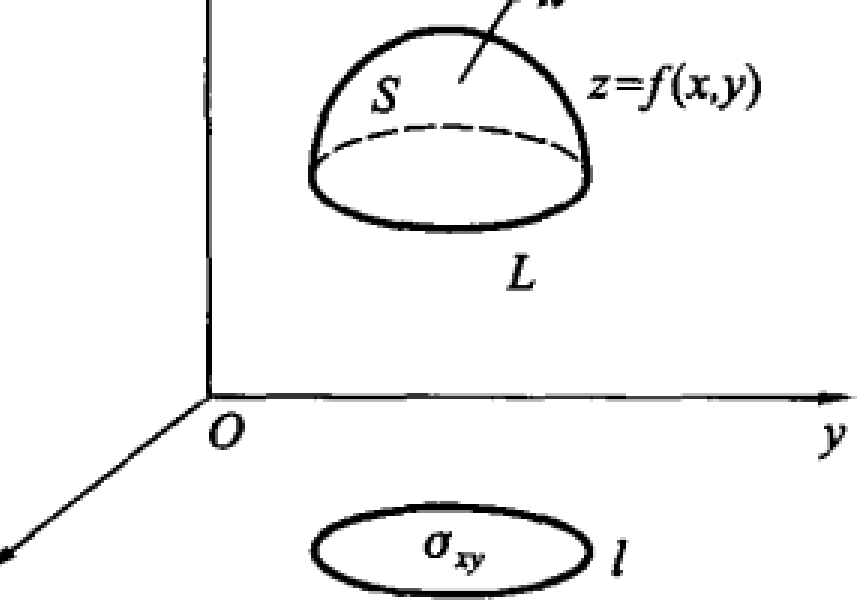
\includegraphics[width=\textwidth]{work/figures/fig22-12}\caption{\relax}\label{fig:22-12}
\end{minipage}\hfill
\begin{minipage}[c]{0.34\textwidth}\centering
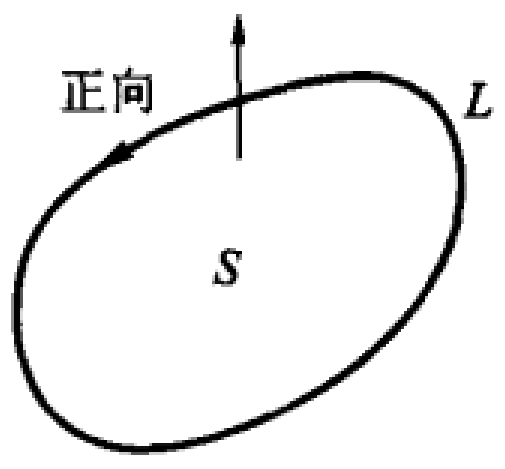
\includegraphics[width=\textwidth]{work/figures/fig22-13}\caption{\relax}\label{fig:22-13}
\end{minipage}
\end{figure}

\begin{proof}
先证
\[
\iint_{S}\frac{\partial P}{\partial z}\mathrm{d}z\mathrm{d}x-\frac{\partial P}{\partial y}\mathrm{d}x\mathrm{d}y=\oint_{L}P\mathrm{d}x.
\]
设曲面 $S$ 的方程为 $z=f(x,y)$，它在 $Oxy$ 面上的投影为 $\sigma_{xy}$，与过 $\sigma_{xy}$ 的点且平行于 $z$ 轴的直线只交于一点．$L$ 是 $S$ 的边界，它在 $Oxy$ 面上的投影为 $l$．取 $S$ 的上侧为正侧，则单位法向量为
\[
\bm{n}=(\cos\alpha,\cos\beta,\cos\gamma)=\frac{1}{\sqrt{\left(\dfrac{\partial z}{\partial x}\right)^{2}+\left(\dfrac{\partial z}{\partial y}\right)^{2}+1}}\left(-\frac{\partial z}{\partial x},-\frac{\partial z}{\partial y},1\right).
\]
因此
\[
\frac{\partial z}{\partial x}=-\frac{\cos\alpha}{\cos\gamma},\quad\frac{\partial z}{\partial y}=-\frac{\cos\beta}{\cos\gamma}.
\]
因为 $L$ 在曲面 $z=f(x,y)$ 上，所以由格林公式，有
\[
\begin{aligned}
\oint_{L}P(x,y,z)\mathrm{d}x&=\oint_{l}P(x,y,z(x,y))\mathrm{d}x\\
&=-\iint_{\sigma_{xy}}\left(\frac{\partial P}{\partial y}+\frac{\partial P}{\partial z}\frac{\partial z}{\partial y}\right)\mathrm{d}x\mathrm{d}y\\
&=-\iint_{\sigma_{xy}}\left(\frac{\partial P}{\partial y}-\frac{\partial P}{\partial z}\frac{\cos\beta}{\cos\gamma}\right)\mathrm{d}x\mathrm{d}y\\
&=\iint_{\sigma_{xy}}\left(\frac{\partial P}{\partial z}\cos\beta-\frac{\partial P}{\partial y}\cos\gamma\right)\frac{\mathrm{d}x\mathrm{d}y}{\cos\gamma}\\
&=\iint_{S}\left(\frac{\partial P}{\partial z}\cos\beta-\frac{\partial P}{\partial y}\cos\gamma\right)\mathrm{d}S\\
&=\iint_{S}\frac{\partial P}{\partial z}\mathrm{d}z\mathrm{d}x-\frac{\partial P}{\partial y}\mathrm{d}x\mathrm{d}y.
\end{aligned}
\]
同理可证
\[
\oint_{L}Q\mathrm{d}y=\iint_{S}\frac{\partial Q}{\partial x}\mathrm{d}x\mathrm{d}y-\frac{\partial Q}{\partial z}\mathrm{d}y\mathrm{d}z,
\]
\[
\oint_{L}R\mathrm{d}z=\iint_{S}\frac{\partial R}{\partial y}\mathrm{d}y\mathrm{d}z-\frac{\partial R}{\partial x}\mathrm{d}z\mathrm{d}x.
\]
把三个式子加起来，便得斯托克斯公式．定理~\ref{thm:22-3} 证完．
\end{proof}

斯托克斯公式建立了函数在空间曲面 $S$ 上的第二型曲面积分与其``原函数''在 $S$ 的边界曲线 $L$ 上的第二型曲线积分之间的联系，因此也是牛顿－莱布尼茨公式的一种高维的推广．利用两种曲面积分之间的关系，常把它写成如下便于记忆的形式：
\[
\begin{aligned}
\oint_{L}P\mathrm{d}x+Q\mathrm{d}y+R\mathrm{d}z&=\iint_{S}\begin{vmatrix}\mathrm{d}y\mathrm{d}z&\mathrm{d}z\mathrm{d}x&\mathrm{d}x\mathrm{d}y\\[3pt]\dfrac{\partial}{\partial x}&\dfrac{\partial}{\partial y}&\dfrac{\partial}{\partial z}\\[3pt] P&Q&R\end{vmatrix}\\
&=\iint_{S}\begin{vmatrix}\cos\alpha&\cos\beta&\cos\gamma\\[3pt]\dfrac{\partial}{\partial x}&\dfrac{\partial}{\partial y}&\dfrac{\partial}{\partial z}\\[3pt] P&Q&R\end{vmatrix}\mathrm{d}S.
\end{aligned}
\]
不难看出，格林公式是斯托克斯公式的特殊情形．当 $L$ 是 $Oxy$ 平面上的闭曲线时，$\mathrm{d}z=0$．取 $S$ 为 $Oxy$ 面上由 $L$ 围成的区域，则 $S$ 在 $Oyz$ 和 $Ozx$ 平面上的投影为零，因此对 $\mathrm{d}y\mathrm{d}z$，$\mathrm{d}z\mathrm{d}x$ 的积分为 $0$，这时斯托克斯公式化为格林公式
\[
\oint_{L}P\mathrm{d}x+Q\mathrm{d}y=\iint_{S}\begin{vmatrix}\dfrac{\partial}{\partial x}&\dfrac{\partial}{\partial y}\\[4pt] P&Q\end{vmatrix}\mathrm{d}x\mathrm{d}y=\iint_{S}\left(\frac{\partial Q}{\partial x}-\frac{\partial P}{\partial y}\right)\mathrm{d}x\mathrm{d}y.
\]

\begin{example}\label{ex:22-1-5}
求 $I=\displaystyle\oint_{L}(y-z)\mathrm{d}x+(z-x)\mathrm{d}y+(x-y)\mathrm{d}z$，其中 $L$ 是柱面 $x^{2}+y^{2}=a^{2}$ 与平面 $\dfrac{x}{a}+\dfrac{z}{h}=1$ 的交线（$a,h>0$），从 $x$ 轴正向看去沿逆时针方向（图~\ref{fig:22-14}）．
\end{example}

\begin{figure}[htbp]
\centering
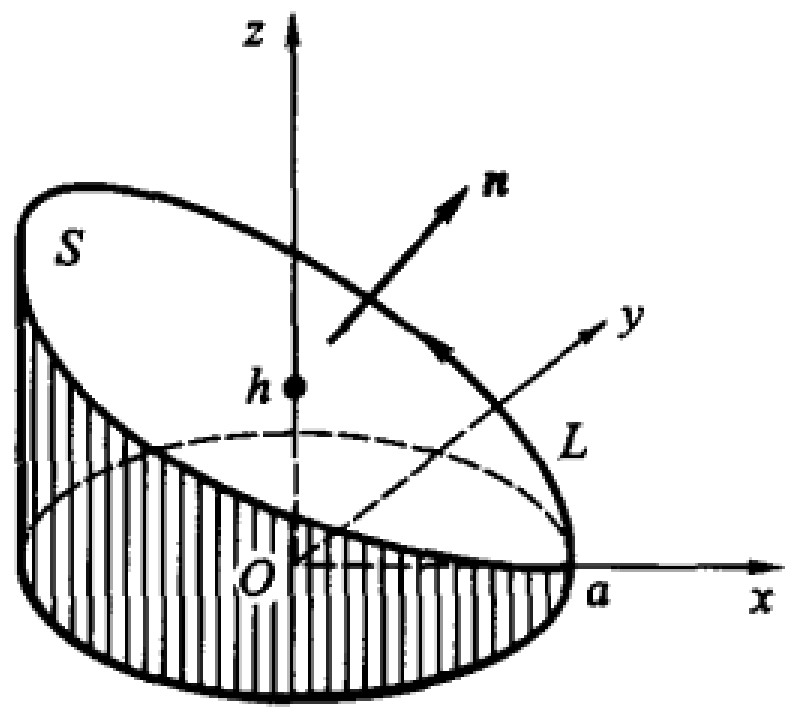
\includegraphics[width=0.28\textwidth]{work/figures/fig22-14}\caption{\relax}\label{fig:22-14}
\end{figure}

\begin{proof}[解法 1]
取平面 $\dfrac{x}{a}+\dfrac{z}{h}=1$ 上由交线围成的平面块为 $S$，并注意 $S$ 在 $Ozx$ 面上的投影为零，即 $\mathrm{d}z\mathrm{d}x=0$，由斯托克斯公式得
\[
\begin{aligned}
I&=\iint_{S}\begin{vmatrix}\mathrm{d}y\mathrm{d}z&\mathrm{d}z\mathrm{d}x&\mathrm{d}x\mathrm{d}y\\[3pt]\dfrac{\partial}{\partial x}&\dfrac{\partial}{\partial y}&\dfrac{\partial}{\partial z}\\[3pt] y-z&z-x&x-y\end{vmatrix}\\
&=2\iint_{S}\mathrm{d}y\mathrm{d}z+\mathrm{d}x\mathrm{d}y=-2\iint_{D_{yz}}\mathrm{d}y\mathrm{d}z-2\iint_{D_{xy}}\mathrm{d}x\mathrm{d}y\\
&=-2(\pi ah+\pi a^{2})=-2\pi a(h+a).
\end{aligned}
\]
最后一个等式是因为 $D_{yz}$ 是半轴分别为 $a$ 与 $h$ 的椭圆，其面积为 $\pi ah$，而 $D_{xy}$ 是圆 $x^{2}+y^{2}\leqslant a^{2}$，其面积为 $\pi a^{2}$．
\end{proof}

\begin{proof}[解法 2]
取曲面 $S$ 同解法 1，则 $S$ 的单位法向量
\[
\bm{n}=\left(\frac{h}{\sqrt{a^{2}+h^{2}}},0,\frac{a}{\sqrt{a^{2}+h^{2}}}\right)=(\cos\alpha,\cos\beta,\cos\gamma)
\]
是常向量，$S$ 是半轴分别为 $a$ 和 $\sqrt{a^{2}+h^{2}}$ 的椭圆．因此
\[
\begin{aligned}
I&=\iint_{S}\begin{vmatrix}\cos\alpha&\cos\beta&\cos\gamma\\[3pt]\dfrac{\partial}{\partial x}&\dfrac{\partial}{\partial y}&\dfrac{\partial}{\partial z}\\[3pt] y-z&z-x&x-y\end{vmatrix}\mathrm{d}S\\
&=-2\iint_{S}(\cos\alpha+\cos\gamma)\mathrm{d}S=-2\frac{a+h}{\sqrt{a^{2}+h^{2}}}\iint_{S}\mathrm{d}S\\
&=-2\frac{a+h}{\sqrt{a^{2}+h^{2}}}\pi a\sqrt{a^{2}+h^{2}}=-2\pi a(h+a).
\end{aligned}
\]
\end{proof}

\begin{proof}[解法 3]
也可以直接用线积分的计算公式．曲线 $L$ 的参数方程为
\[
x=a\cos t,\quad y=a\sin t,\quad z=h(1-\cos t),\ 0\leqslant t\leqslant 2\pi,
\]
则
\[
\begin{aligned}
I&=\int_{0}^{2\pi}\left\{\left[a\sin t-h(1-\cos t)\right](-a\sin t)\right.\\
&\quad\left.+\left[h(1-\cos t)-a\cos t\right]a\cos t+a(\cos t-\sin t)h\sin t\right\}\mathrm{d}t\\
&=\int_{0}^{2\pi}\left(-a^{2}-ah+ah\sin t+ah\cos t\right)\mathrm{d}t\\
&=-2\pi a(a+h).
\end{aligned}
\]
\end{proof}

到此为止，我们对各种积分的概念及其相互间的关系已经有了较完整的认识．二重积分、三重积分、两种类型的曲线积分和两种类型的曲面积分，它们来自不同的物理背景，抽象出不同的数学定义，但却有着奇妙的联系．格林公式、高斯公式和斯托克斯公式描述了这些联系，反映出的共同点是它们都给出空间某形体的积分与其边界上的积分的关系．它们都是牛顿－莱布尼茨公式的推广．

\begin{xiti}
\item 应用格林公式计算下列积分：
\begin{ziti}
\item $\displaystyle\oint_{L}xy^{2}\mathrm{d}y-x^{2}y\mathrm{d}x$，其中 $L$ 为椭圆 $\dfrac{x^{2}}{a^{2}}+\dfrac{y^{2}}{b^{2}}=1$，取正向；
\item $\displaystyle\oint_{L}(x+y)\mathrm{d}x+(x-y)\mathrm{d}y$，$L$ 同 (1)；
\item $\displaystyle\oint_{L}(x+y)^{2}\mathrm{d}x-(x^{2}+y^{2})\mathrm{d}y$，$L$ 是顶点为 $A(1,1)$，$B(3,2)$，$C(2,5)$ 的三角形的边界，取正向；
\item $\displaystyle\oint_{L}(x^{2}+y^{3})\mathrm{d}x-(x^{3}-y^{2})\mathrm{d}y$，$L$ 为 $x^{2}+y^{2}=1$，取正向；
\item $\displaystyle\oint_{L}\mathrm{e}^{y}\sin x\,\mathrm{d}x+\mathrm{e}^{-x}\sin y\,\mathrm{d}y$，$L$ 为矩形 $a\leqslant x\leqslant b$，$c\leqslant y\leqslant d$ 的边界，取正向；
\item $\displaystyle\oint_{L}\left[\left(y\sin xy+\cos(x+y)\right)\mathrm{d}x+\left(x\sin xy+\cos(x+y)\right)\mathrm{d}y\right]$，其中 $L$ 是任意逐段光滑闭曲线．
\end{ziti}
\item 利用格林公式计算下列曲线所围图形的面积：
\begin{ziti}
\item 双纽线 $r^{2}=a^{2}\cos 2\theta$；
\item 笛卡儿叶形线 $x^{3}+y^{3}=3axy$（$a>0$）；
\item $x=a(1+\cos^{2}t)\sin t$，$y=a\sin^{2}t\cos t$，$0\leqslant t\leqslant 2\pi$．
\end{ziti}
\item 利用高斯公式求下列积分：
\begin{ziti}
\item $\displaystyle\iint_{S}x^{2}\mathrm{d}y\mathrm{d}z+y^{2}\mathrm{d}z\mathrm{d}x+z^{2}\mathrm{d}x\mathrm{d}y$，其中（a）$S$ 为立方体 $0\leqslant x,y,z\leqslant a$ 的边界曲面外侧；（b）$S$ 为锥面 $x^{2}+y^{2}=z^{2}$（$0\leqslant z\leqslant h$），下侧．
\item $\displaystyle\iint_{S}x^{3}\mathrm{d}y\mathrm{d}z+y^{3}\mathrm{d}z\mathrm{d}x+z^{3}\mathrm{d}x\mathrm{d}y$，其中 $S$ 是单位球面的外侧；
\item 设 $S$ 是上半球面 $z=\sqrt{a^{2}-x^{2}-y^{2}}$ 的上侧，求（a）$\displaystyle\iint_{S}x\,\mathrm{d}y\mathrm{d}z+y\,\mathrm{d}z\mathrm{d}x+z\,\mathrm{d}x\mathrm{d}y$，（b）$\displaystyle\iint_{S}xz^{2}\mathrm{d}y\mathrm{d}z+(x^{2}y-z^{2})\mathrm{d}z\mathrm{d}x+(2xy+y^{2}z)\mathrm{d}x\mathrm{d}y$；
\item $\displaystyle\iint_{S}(x-y^{2}+z^{2})\mathrm{d}y\mathrm{d}z+(y-z^{2}+x^{2})\mathrm{d}z\mathrm{d}x+(z-x^{2}+y^{2})\mathrm{d}x\mathrm{d}y$，$S$ 是 $(x-a)^{2}+(y-b)^{2}+(z-c)^{2}=R^{2}$ 的外侧．
\end{ziti}
\item 用斯托克斯公式计算下列积分：
\begin{ziti}
\item $\displaystyle\oint_{L}x^{2}y^{3}\mathrm{d}x+\mathrm{d}y+z\mathrm{d}z$，其中（a）$L$ 为圆周 $x^{2}+y^{2}=a^{2}$，$z=0$，方向是逆时针；（b）$L$ 为 $y^{2}+z^{2}=1$，$x=y$ 所交的椭圆，从 $x$ 轴正向看去，按逆时针方向；
\item $\displaystyle\oint_{L}(y-z)\mathrm{d}x+(z-x)\mathrm{d}y+(x-y)\mathrm{d}z$，$L$ 是从 $(a,0,0)$ 经 $(0,a,0)$ 至 $(0,0,a)$ 回到 $(a,0,0)$ 的三角形；
\item $\displaystyle\oint_{L}(y^{2}+z^{2})\mathrm{d}x+(x^{2}+z^{2})\mathrm{d}y+(x^{2}+y^{2})\mathrm{d}z$，其中（a）$L$ 为 $x+y+z=1$ 与三坐标平面的交线，其方向与所围平面区域上侧构成右手法则，（b）$L$ 是曲线 $x^{2}+y^{2}+z^{2}=2Rx$，$x^{2}+y^{2}=2rx$（$0<r<R$，$z>0$），它的方向与所围曲面的上侧构成右手法则；
\item $\displaystyle\oint_{L}y\,\mathrm{d}x+z\,\mathrm{d}y+x\,\mathrm{d}z$，$L$ 是 $x^{2}+y^{2}+z^{2}=a^{2}$，$x+y+z=0$，从 $x$ 轴正向看去圆周是逆时针方向．
\end{ziti}
\item 设 $L$ 为平面上封闭曲线，$l$ 为平面上任意方向，证明
\[
\oint_{L}\cos(\bm{n},l)\mathrm{d}s=0,
\]
其中 $\bm{n}$ 是 $L$ 的外法线方向．
\item 设 $S$ 是封闭曲面，$l$ 为任意固定方向，证明
\[
\oiint_{S}\cos(\bm{n},l)\mathrm{d}S=0.
\]
\item 求 $I=\displaystyle\oint_{L}\left[x\cos(\bm{n},x)+y\cos(\bm{n},y)\right]\mathrm{d}s$，$L$ 为包围有界区域 $D$ 的光滑闭曲线，$\bm{n}$ 为 $L$ 的外法向．
\item 证明高斯积分
\[
\oint_{L}\frac{\cos(\bm{r},\bm{n})}{r}\mathrm{d}s=0,
\]
其中 $L$ 是平面上一单连通区域 $\sigma$ 的边界，而 $r$ 是 $L$ 上一点到 $\sigma$ 外某一定点的距离，$\bm{n}$ 是 $L$ 的外法线方向．又若 $r$ 表示 $L$ 上一点到 $\sigma$ 内某一定点的距离，则这个积分之值等于 $2\pi$．
\item 计算高斯积分
\[
\iint_{S}\frac{\cos(\bm{r},\bm{n})}{r^{2}}\mathrm{d}S,
\]
其中 $S$ 为简单封闭光滑曲面，$\bm{n}$ 为曲面 $S$ 上在点 $(\xi,\eta,\zeta)$ 处的外法向，$\bm{r}=(\xi-x)\bm{i}+(\eta-y)\bm{j}+(\zeta-z)\bm{k}$，$r=|\bm{r}|$．试对下列两种情形进行讨论：（1）曲面 $S$ 包围的区域不含 $(x,y,z)$ 点；（2）曲面 $S$ 包围的区域含 $(x,y,z)$ 点．
\item 求证：
\[
\iiint_{V}\frac{\mathrm{d}x\mathrm{d}y\mathrm{d}z}{r}=\frac{1}{2}\oiint_{S}\cos(\bm{r},\bm{n})\mathrm{d}S,
\]
其中 $S$ 是包围 $V$ 的分片光滑封闭曲面，$\bm{n}$ 为 $S$ 的外法线方向，$\bm{r}=(x,y,z)$，$r=|\bm{r}|$．分下列两种情形进行讨论：（1）$V$ 中不含原点 $(0,0,0)$；（2）$V$ 中含原点 $(0,0,0)$ 时，令
\[
\iiint_{V}\frac{\mathrm{d}x\mathrm{d}y\mathrm{d}z}{r}=\lim_{\varepsilon\to 0^{+}}\iiint_{V-V_{\varepsilon}}\frac{\mathrm{d}x\mathrm{d}y\mathrm{d}z}{r},
\]
其中 $V_{\varepsilon}$ 是以原点为心，以 $\varepsilon$ 为半径的球．
\item 利用高斯公式变换以下积分：
\begin{ziti}
\item $\displaystyle\iint_{S}xy\,\mathrm{d}x\mathrm{d}y+xz\,\mathrm{d}z\mathrm{d}x+yz\,\mathrm{d}y\mathrm{d}z$；
\item $\displaystyle\iint_{S}\left(\frac{\partial u}{\partial x}\cos\alpha+\frac{\partial u}{\partial y}\cos\beta+\frac{\partial u}{\partial z}\cos\gamma\right)\mathrm{d}S$，其中 $\cos\alpha,\cos\beta,\cos\gamma$ 是曲面的外法线方向余弦．
\end{ziti}
\item 设 $u(x,y)$，$v(x,y)$ 是具有二阶连续偏导数的函数，并设
\[
\Delta u=\frac{\partial^{2}u}{\partial x^{2}}+\frac{\partial^{2}u}{\partial y^{2}}.
\]
证明：
\begin{ziti}
\item $\displaystyle\iint_{\sigma}\Delta u\,\mathrm{d}x\mathrm{d}y=\oint_{l}\frac{\partial u}{\partial n}\,\mathrm{d}s$；
\item $\displaystyle\iint_{\sigma}v\Delta u\,\mathrm{d}x\mathrm{d}y=-\iint_{\sigma}\left(\frac{\partial u}{\partial x}\frac{\partial v}{\partial x}+\frac{\partial u}{\partial y}\frac{\partial v}{\partial y}\right)\mathrm{d}x\mathrm{d}y+\oint_{l}v\frac{\partial u}{\partial n}\mathrm{d}s$；
\item $\displaystyle\iint_{\sigma}\left(u\Delta v-v\Delta u\right)\mathrm{d}x\mathrm{d}y=-\oint_{l}\left(v\frac{\partial u}{\partial n}-u\frac{\partial v}{\partial n}\right)\mathrm{d}s$.
\end{ziti}
其中 $\sigma$ 为闭曲线 $l$ 所围的平面区域，$\dfrac{\partial u}{\partial n}$，$\dfrac{\partial v}{\partial n}$ 为沿 $l$ 外法线的方向导数．
\item 设 $\Delta u=\dfrac{\partial^{2}u}{\partial x^{2}}+\dfrac{\partial^{2}u}{\partial y^{2}}+\dfrac{\partial^{2}u}{\partial z^{2}}$，$S$ 是 $V$ 的边界曲面，证明：
\begin{ziti}
\item $\displaystyle\iiint_{V}\Delta u\,\mathrm{d}x\mathrm{d}y\mathrm{d}z=\iint_{S}\frac{\partial u}{\partial n}\,\mathrm{d}S$；
\item $\displaystyle\iint_{S}u\frac{\partial u}{\partial n}\mathrm{d}S=\iiint_{V}\left[\left(\frac{\partial u}{\partial x}\right)^{2}+\left(\frac{\partial u}{\partial y}\right)^{2}+\left(\frac{\partial u}{\partial z}\right)^{2}\right]\mathrm{d}x\mathrm{d}y\mathrm{d}z+\iiint_{V}u\Delta u\,\mathrm{d}x\mathrm{d}y\mathrm{d}z$.
\end{ziti}
式中 $u$ 在 $V$ 及其边界曲面 $S$ 上有连续的二阶偏导数，$\dfrac{\partial u}{\partial n}$ 为沿曲面 $S$ 的外法线的方向导数．
\item 计算下列曲面积分：
\begin{ziti}
\item $\displaystyle\iint_{S}(x^{2}-y^{2})\mathrm{d}y\mathrm{d}z+(y^{2}-z^{2})\mathrm{d}z\mathrm{d}x+2z(y-x)\mathrm{d}x\mathrm{d}y$，其中 $S$ 是 $\dfrac{x^{2}}{a^{2}}+\dfrac{y^{2}}{b^{2}}+\dfrac{z^{2}}{c^{2}}=1$（$z\geqslant 0$）下侧；
\item $\displaystyle\iint_{S}(x+\cos y)\,\mathrm{d}y\mathrm{d}z+(y+\cos z)\,\mathrm{d}z\mathrm{d}x+(z+\cos x)\,\mathrm{d}x\mathrm{d}y$，$S$ 是立体 $\Omega$ 的边界面，而立体 $\Omega$ 由 $x+y+z=1$ 和三坐标面围成；
\item $\displaystyle\iint_{S}\bm{F}\cdot\bm{n}\,\mathrm{d}S$，其中 $\bm{F}=x^{3}\bm{i}+y^{3}\bm{j}+z^{3}\bm{k}$，$\bm{n}$ 是 $S$ 的外法向，$S$ 为 $x^{2}+y^{2}+z^{2}=a^{2}(z\geqslant 0)$ 上侧；
\item $\displaystyle\iint_{S}\left(\frac{x^{3}}{a^{2}}+yz\right)\mathrm{d}y\mathrm{d}z+\left(\frac{y^{3}}{b^{2}}+z^{3}x^{2}\right)\mathrm{d}z\mathrm{d}x+\left(\frac{z^{3}}{c^{2}}+x^{3}y^{3}\right)\mathrm{d}x\mathrm{d}y$，$S$ 是 $\dfrac{x^{2}}{a^{2}}+\dfrac{y^{2}}{b^{2}}+\dfrac{z^{2}}{c^{2}}=1$（$x\geqslant 0$）后侧．
\end{ziti}
\item 证明由曲面 $S$ 所包围的体积等于
\[
V=\frac{1}{3}\iint_{S}\left(x\cos\alpha+y\cos\beta+z\cos\gamma\right)\mathrm{d}S,
\]
式中 $\cos\alpha$，$\cos\beta$，$\cos\gamma$ 为曲面 $S$ 的外法线的方向余弦．
\item 若 $L$ 是平面 $x\cos\alpha+y\cos\beta+z\cos\gamma-p=0$ 上逐段光滑的闭曲线，它所包围区域的面积为 $S$，求
\[
\oint_{L}\begin{vmatrix}\mathrm{d}x&\mathrm{d}y&\mathrm{d}z\\ \cos\alpha&\cos\beta&\cos\gamma\\ x&y&z\end{vmatrix},
\]
其中 $L$ 依正向进行．
\item 设 $P$，$Q$，$R$ 有连续偏导数，且对任意光滑闭曲面 $S$，有
\[
\iint_{S}P\mathrm{d}y\mathrm{d}z+Q\mathrm{d}z\mathrm{d}x+R\mathrm{d}x\mathrm{d}y=0.
\]
证明 $\dfrac{\partial P}{\partial x}+\dfrac{\partial Q}{\partial y}+\dfrac{\partial R}{\partial z}=0$．
\item 设 $P(x,y)$，$Q(x,y)$ 在全平面上有连续偏导数，而且以任意点 $(x_{0},y_{0})$ 为中心，以任意正数 $r$ 为半径的上半圆 $l$：$x=x_{0}+r\cos\theta$，$y=y_{0}+r\sin\theta$（$0\leqslant\theta\leqslant\pi$），恒有
\[
\int_{l}P(x,y)\mathrm{d}x+Q(x,y)\mathrm{d}y=0,
\]
求证：$P(x,y)=0$，$\dfrac{\partial Q}{\partial x}=0$．
\end{xiti}

\section{积分与路径无关}

考虑积分
\[
\int_{L}\frac{x\mathrm{d}y-y\mathrm{d}x}{x^{2}+y^{2}}.
\]
对于圆 $x=a\cos\theta$，$y=a\sin\theta$，记 $L_{1}$ 为上半圆周，$L_{2}$ 为下半圆周，方向都是从 $(-a,0)$ 点到 $(a,0)$ 点．则
\[
\begin{aligned}
\int_{L_{1}}\frac{x\mathrm{d}y-y\mathrm{d}x}{x^{2}+y^{2}}&=-\pi,\\
\int_{L_{2}}\frac{x\mathrm{d}y-y\mathrm{d}x}{x^{2}+y^{2}}&=\pi.
\end{aligned}
\]
它表明尽管 $L_{1}$ 与 $L_{2}$ 有相同的起点和相同的终点，但由于路径不同，积分值也不同，即积分与路径有关．又若 $L$ 是起点为 $(-a,0)$，终点为 $(a,0)$ 的光滑曲线，且与 $L_{1}$ 构成不包围原点的闭曲线，由格林公式有
\[
\left(\int_{L_{1}}-\int_{L}\right)\frac{x\mathrm{d}y-y\mathrm{d}x}{x^{2}+y^{2}}=0,
\]
即 $\displaystyle\int_{L}\frac{x\mathrm{d}y-y\mathrm{d}x}{x^{2}+y^{2}}=\int_{L_{1}}\frac{x\mathrm{d}y-y\mathrm{d}x}{x^{2}+y^{2}}=-\pi$．
\begin{figure}[htbp]
\centering
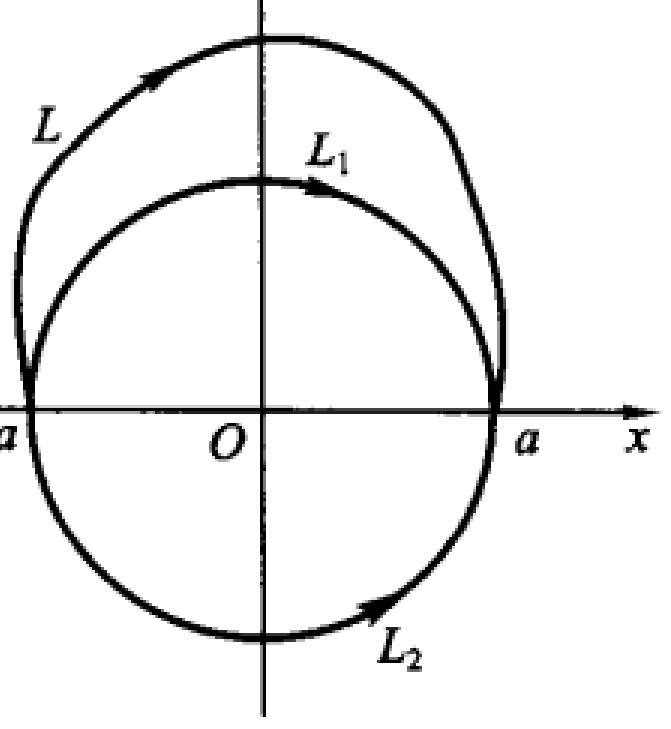
\includegraphics[width=0.28\textwidth]{work/figures/fig22-15}\caption{\relax}\label{fig:22-15}
\end{figure}
它又表明从 $(-a,0)$ 出发经上半平面越过 $y$ 轴到 $(a,0)$ 点的任一条光滑曲线的积分与路径无关，积分值都是 $-\pi$．

在什么条件下积分与路径无关呢？

\begin{theorem}\label{thm:22-4}
设 $D$ 是平面单连通区域，函数 $P(x,y)$，$Q(x,y)$ 在 $D$ 上有连续偏导数，则下列四断言等价：
\begin{enumerate}[label=（\arabic*）]
\item 沿 $D$ 中任一逐段光滑的闭曲线 $L$，有 $\displaystyle\oint_{L}P\mathrm{d}x+Q\mathrm{d}y=0$；
\item 对 $D$ 中任一逐段光滑曲线 $L$，曲线积分 $\displaystyle\int_{L}P\mathrm{d}x+Q\mathrm{d}y$ 与路径无关，只与 $L$ 的起点与终点有关；
\item 微分式 $P\mathrm{d}x+Q\mathrm{d}y$ 在 $D$ 内是某函数 $u(x,y)$ 的全微分，即有 $\mathrm{d}u=P\mathrm{d}x+Q\mathrm{d}y$；
\item 在 $D$ 内每一点有 $\dfrac{\partial P}{\partial y}=\dfrac{\partial Q}{\partial x}$．
\end{enumerate}
\end{theorem}

\begin{proof}
（1）$\Rightarrow$（2）．设 $A$、$B$ 是 $D$ 内任意两点，$L_{1}$ 和 $L_{2}$ 是完全含于 $D$ 内的任意两条连结 $A$、$B$ 的逐段光滑曲线，方向都是从 $A$ 到 $B$．于是 $L_{1}$ 与 $L_{2}$ 的反向构成完全含于 $D$ 内的一条闭曲线，由（1）知
\[
\left(\int_{L_{1}}-\int_{L_{2}}\right)P\mathrm{d}x+Q\mathrm{d}y=0,
\]
即
\[
\int_{L_{1}}P\mathrm{d}x+Q\mathrm{d}y=\int_{L_{2}}P\mathrm{d}x+Q\mathrm{d}y,
\]
这表明（2）成立．

（2）$\Rightarrow$（3）．设 $A(x_{0},y_{0})$，$B(x,y)$ 为 $D$ 内的两点，由（2）知，从 $A$ 到 $B$ 的积分只与起点和终点有关，而与路径无关，把起点固定在 $A(x_{0},y_{0})$，则积分便是终点 $(x,y)$ 的函数，记为
\begin{figure}[htbp]
\centering
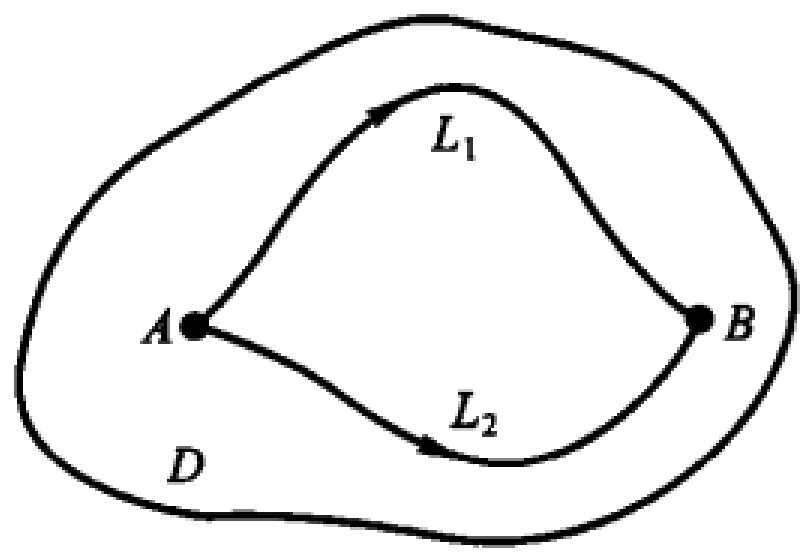
\includegraphics[width=0.28\textwidth]{work/figures/fig22-16}\caption{\relax}\label{fig:22-16}
\end{figure}
\[
u(x,y)=\int_{(x_{0},y_{0})}^{(x,y)}P\mathrm{d}x+Q\mathrm{d}y.
\]
显然 $u(x,y)$ 定义在 $D$ 内，下面要证
\[
\frac{\partial u}{\partial x}=P(x,y),\qquad\frac{\partial u}{\partial y}=Q(x,y).
\]
由于 $B(x,y)$ 是 $D$ 的内点，当 $|\Delta x|$ 充分小时，$(x+\Delta x,y)\in D$．考虑
\[
\begin{aligned}
&u(x+\Delta x,y)-u(x,y)\\
=&\int_{(x_{0},y_{0})}^{(x+\Delta x,y)}P\mathrm{d}x+Q\mathrm{d}y-\int_{(x_{0},y_{0})}^{(x,y)}P\mathrm{d}x+Q\mathrm{d}y.
\end{aligned}
\]
由于积分与路径无关，取从 $(x_{0},y_{0})$ 到 $(x+\Delta x,y)$ 的路径经过 $B(x,y)$ 点，而从 $B(x,y)$ 到 $(x+\Delta x,y)$ 的路径则取连结两点的直线段，再用积分中值定理，有
\begin{figure}[htbp]
\centering
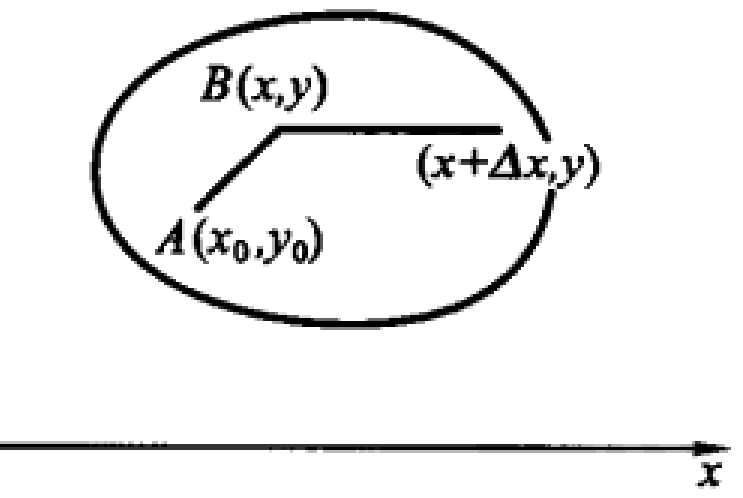
\includegraphics[width=0.28\textwidth]{work/figures/fig22-17}\caption{\relax}\label{fig:22-17}
\end{figure}
\[
\begin{aligned}
&u(x+\Delta x,y)-u(x,y)\\
=&\int_{(x,y)}^{(x+\Delta x,y)}P\mathrm{d}x+Q\mathrm{d}y=\int_{(x,y)}^{(x+\Delta x,y)}P(x,y)\mathrm{d}x\\
=&\int_{x}^{x+\Delta x}P(x,y)\mathrm{d}x=P(\xi,y)\Delta x,
\end{aligned}
\]
其中 $\xi$ 在 $x$ 与 $x+\Delta x$ 之间．因为 $P(x,y)$ 在 $D$ 内连续，所以
\[
\begin{aligned}
\frac{\partial u}{\partial x}&=\lim_{\Delta x\to 0}\frac{u(x+\Delta x,y)-u(x,y)}{\Delta x}\\
&=\lim_{\Delta x\to 0}P(\xi,y)=P(x,y).
\end{aligned}
\]
同理可证 $\dfrac{\partial u}{\partial y}=Q(x,y)$．由 $\dfrac{\partial u}{\partial x}=P(x,y)$ 和 $\dfrac{\partial u}{\partial y}=Q(x,y)$ 都在 $D$ 内连续，知 $u(x,y)$ 在 $D$ 内可微，且有
\[
\mathrm{d}u=\frac{\partial u}{\partial x}\mathrm{d}x+\frac{\partial u}{\partial y}\mathrm{d}y=P(x,y)\mathrm{d}x+Q(x,y)\mathrm{d}y.
\]
（3）$\Rightarrow$（4）．已知 $\mathrm{d}u=P\mathrm{d}x+Q\mathrm{d}y$，因此
\[
\frac{\partial u}{\partial x}=P(x,y),\qquad\frac{\partial u}{\partial y}=Q(x,y),
\]
故
\[
\frac{\partial^{2}u}{\partial x\partial y}=\frac{\partial P}{\partial y},\quad\frac{\partial^{2}u}{\partial y\partial x}=\frac{\partial Q}{\partial x}.
\]
根据 $P$，$Q$ 在 $D$ 内有连续的偏导数，有 $\dfrac{\partial^{2}u}{\partial x\partial y}=\dfrac{\partial^{2}u}{\partial y\partial x}$，即
\[
\frac{\partial P}{\partial y}=\frac{\partial Q}{\partial x}.
\]
（4）$\Rightarrow$（1）．设 $L$ 是完全含于 $D$ 内的任一逐段光滑的闭曲线，$L$ 所围区域为 $\sigma$，$L$ 的方向关于 $\sigma$ 为正向．因为 $D$ 是单连通区域，所以 $\sigma$ 完全含于 $D$ 内，因此在 $\sigma$ 上 $\dfrac{\partial Q}{\partial x}=\dfrac{\partial P}{\partial y}$．故由格林公式，得
\[
\oint_{L}P\mathrm{d}x+Q\mathrm{d}y=\iint_{\sigma}\left(\frac{\partial Q}{\partial x}-\frac{\partial P}{\partial y}\right)\mathrm{d}x\mathrm{d}y=0.
\]
定理~\ref{thm:22-4} 证完．
\end{proof}

回头看看定理的证明，不难发现，``$D$ 是单连通区域''的条件只在（4）$\Rightarrow$（1）的证明中用到．可以证明，若 $D$ 是复连通区域，则（1）、（2）、（3）仍是等价的（证明留给读者）．但对（1）或（2）或（3）来说，断言（4）只是必要的，而不是充分的，即当（4）成立时，未必有（1）、（2）、（3）成立．在这里，单连通区域的条件是重要的．例如本节开头的例子
\[
\int_{L}\frac{x\mathrm{d}y-y\mathrm{d}x}{x^{2}+y^{2}}=\int_{L}P\mathrm{d}x+Q\mathrm{d}y.
\]
我们已经计算过，从 $(-a,0)$ 出发沿上半圆周 $L_{1}$ 到 $(a,0)$ 点的积分不等于沿下半圆周 $L_{2}$ 到 $(a,0)$ 点的积分．其原因就在于 $L_{1}$ 和 $L_{2}$ 所围的区域包含了坐标原点，而 $\dfrac{\partial Q}{\partial x}=\dfrac{\partial P}{\partial y}$ 在原点 $(0,0)$ 不成立．换句话说，既包含 $L_{1}$ 和 $L_{2}$，又能使 $\dfrac{\partial Q}{\partial x}=\dfrac{\partial P}{\partial y}$ 处处成立的区域只能是复连通区域．这个例子表明，在复连通区域 $D$ 上，尽管条件（4）成立，也不能保证沿 $D$ 内的光滑曲线的积分与路径无关．

使 $\dfrac{\partial Q}{\partial x}=\dfrac{\partial P}{\partial y}$ 不成立的点称为积分 $\displaystyle\int_{L}P\mathrm{d}x+Q\mathrm{d}y$ 的\emph{奇点}．在单连通区域中把这些``奇点''挖去，则单连通性受到破坏而成为复连通区域 $D$，但在复连通区域 $D$ 中条件 $\dfrac{\partial Q}{\partial x}=\dfrac{\partial P}{\partial y}$ 却处处得到满足．这时有下述结论：

（1）对 $D$ 内任意一条不包围奇点的闭曲线 $L$，有
\[
\oint_{L}P\mathrm{d}x+Q\mathrm{d}y=0.
\]
（2）环绕某一奇点的任意两条简单闭曲线 $L_{1}$ 和 $L_{2}$ 的正向的积分相等，即
\[
\oint_{L_{1}}P\mathrm{d}x+Q\mathrm{d}y=\oint_{L_{2}}P\mathrm{d}x+Q\mathrm{d}y.
\]
这个公共值称为该奇点的\emph{循环常数}．
\begin{figure}[htbp]
\centering
\begin{minipage}[c]{0.44\textwidth}\centering
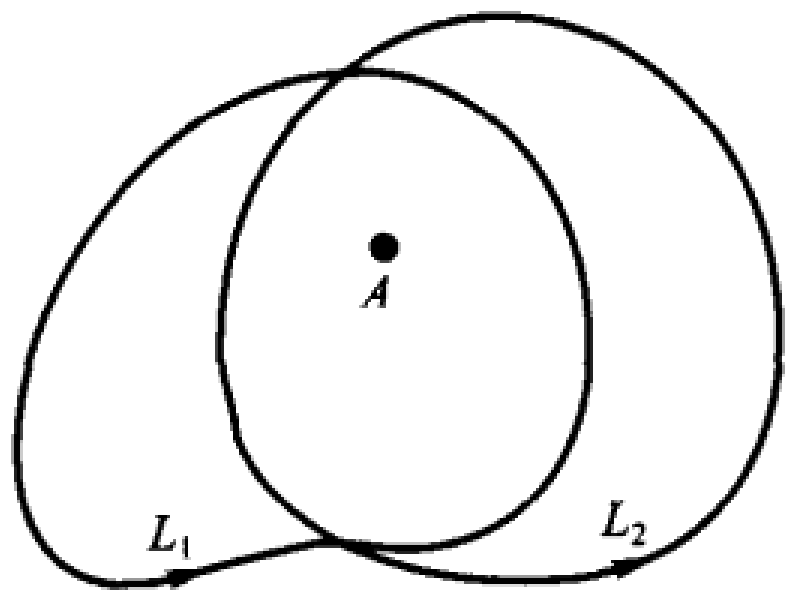
\includegraphics[width=\textwidth]{work/figures/fig22-18}\caption{\relax}\label{fig:22-18}
\end{minipage}\hfill
\begin{minipage}[c]{0.30\textwidth}\centering
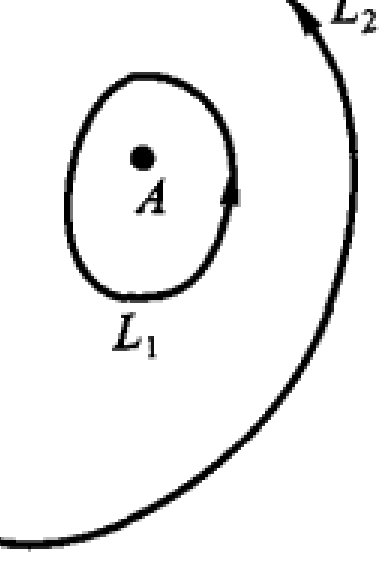
\includegraphics[width=\textwidth]{work/figures/fig22-19}\caption{\relax}\label{fig:22-19}
\end{minipage}
\end{figure}

事实上，若 $L$ 是 $D$ 内任意一条不包围奇点的闭曲线，则在 $L$ 包围的区域 $\sigma$ 内处处成立 $\dfrac{\partial Q}{\partial x}=\dfrac{\partial P}{\partial y}$，由格林公式即证得（1）成立．若 $L_{1}$ 和 $L_{2}$ 是两条包围奇点的简单闭曲线，且方向相同，记 $L_{1}$ 的反方向为 $L_{1}^{-}$，$\sigma$ 是 $L_{1}^{-}$ 和 $L_{2}$ 所围的不含奇点的平面区域（图~\ref{fig:22-18} 和图~\ref{fig:22-19}），则由格林公式知
\[
\left(\int_{L_{1}^{-}}+\int_{L_{2}}\right)P\mathrm{d}x+Q\mathrm{d}y=\iint_{\sigma}\left(\frac{\partial Q}{\partial x}-\frac{\partial P}{\partial y}\right)\mathrm{d}x\mathrm{d}y=0,
\]
即
\[
\int_{L_{1}}P\mathrm{d}x+Q\mathrm{d}y=\int_{L_{2}}P\mathrm{d}x+Q\mathrm{d}y.
\]
从前面的例子可知，积分 $I=\displaystyle\oint_{L}\frac{x\mathrm{d}y-y\mathrm{d}x}{x^{2}+y^{2}}$ 只有一个奇点 $(0,0)$，它的循环常数是 $2\pi$．因此，若 $L$ 是不包围 $(0,0)$ 点的闭曲线，则 $I=0$；若 $L$ 是包围 $(0,0)$ 点的简单闭曲线的正向，则 $I=2\pi$．

进一步还有下述结论：

（3）环绕某一奇点 $n$ 圈的光滑闭曲线 $L$，其中 $n_{1}$ 圈是正向，$n_{2}$ 圈是负向，$n_{1}+n_{2}=n$，则积分 $I=\displaystyle\oint_{L}P\mathrm{d}x+Q\mathrm{d}y$ 等于该点循环常数的 $n_{1}-n_{2}$ 倍．图~\ref{fig:22-20} 是绕 $A$ 两圈的例子．
\begin{figure}[htbp]
\centering
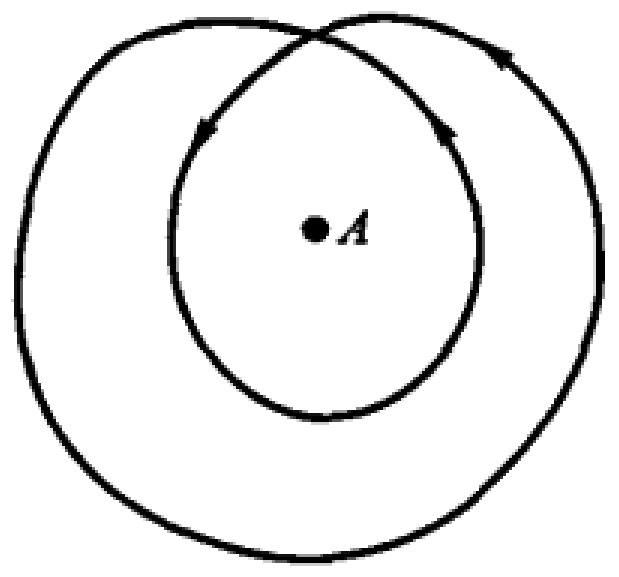
\includegraphics[width=0.22\textwidth]{work/figures/fig22-20}\caption{\relax}\label{fig:22-20}
\end{figure}

（4）若不自相交光滑闭曲线 $L$ 包围了 $k$ 个奇点，则沿 $L$ 正向的积分 $I=\displaystyle\oint_{L}P\mathrm{d}x+Q\mathrm{d}y$ 等于这 $k$ 个奇点的循环常数之和．

\begin{example}\label{ex:22-2-1}
求 $I=\displaystyle\oint_{L}\frac{x\,\mathrm{d}x+y\,\mathrm{d}y}{\sqrt{x^{2}+y^{2}}}$，其中 $L$ 是任意一条不经过原点的闭曲线．
\end{example}

\begin{proof}[解]
记
\[
P(x,y)=\frac{x}{\sqrt{x^{2}+y^{2}}},\quad Q(x,y)=\frac{y}{\sqrt{x^{2}+y^{2}}},
\]
则
\[
\frac{\partial Q}{\partial x}=\frac{\partial P}{\partial y}=-\frac{xy}{\left(x^{2}+y^{2}\right)^{3/2}},\quad(x,y)\neq(0,0).
\]
这说明积分只有一个奇点 $(0,0)$．为求其循环常数，取 $l$ 为单位圆 $x^{2}+y^{2}=1$ 的正向，则
\[
\oint_{l}\frac{x\mathrm{d}x+y\mathrm{d}y}{\sqrt{x^{2}+y^{2}}}=\oint_{l}x\mathrm{d}x+y\mathrm{d}y=\iint_{\sigma}0\,\mathrm{d}x\mathrm{d}y=0,
\]
其中 $\sigma$ 是 $x^{2}+y^{2}\leqslant 1$，即 $(0,0)$ 点的循环常数为 $0$，故对任意一条不经过原点的闭曲线 $L$，有 $I=0$．
\end{proof}

定理~\ref{thm:22-4} 的（2）、（3）表明，在积分与路径无关的条件下，存在函数 $u(x,y)$，使得 $u(x,y)$ 的全微分就是 $P\mathrm{d}x+Q\mathrm{d}y$，即
\[
\mathrm{d}u(x,y)=P(x,y)\mathrm{d}x+Q(x,y)\mathrm{d}y.
\]
这时我们称函数 $u(x,y)$ 为 $P\mathrm{d}x+Q\mathrm{d}y$ 的\emph{原函数}．在这种情况下，对 $D$ 内任意两点 $A$ 与 $B$，有
\[
\int_{A}^{B}P\mathrm{d}x+Q\mathrm{d}y=\int_{A}^{B}\mathrm{d}u=u(x,y)\bigg|_{A}^{B}=u(B)-u(A).
\]
问题是原函数 $u(x,y)$ 如何求呢？

从定理的证明知道 $P\mathrm{d}x+Q\mathrm{d}y$ 的一个原函数可表为
\[
u(x,y)=\int_{(x_{0},y_{0})}^{(x,y)}P(x,y)\mathrm{d}x+Q(x,y)\mathrm{d}y.
\]
由于积分与路径无关，可以任意地选择一条起点为 $(x_{0},y_{0})$，终点为 $(x,y)$ 且完全含于 $D$ 内的路径．为计算方便，通常是取含于 $D$ 内如图~\ref{fig:22-21} 所示的折线段，这时有
\begin{figure}[htbp]
\centering
\begin{minipage}[c]{0.42\textwidth}\centering
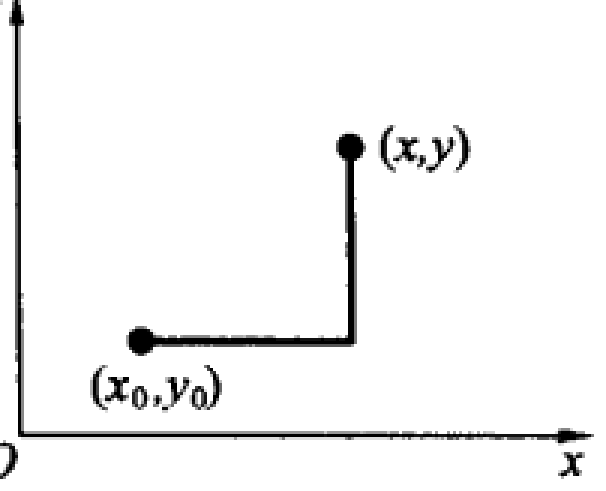
\includegraphics[width=\textwidth]{work/figures/fig22-21a}
\end{minipage}\hfill
\begin{minipage}[c]{0.42\textwidth}\centering
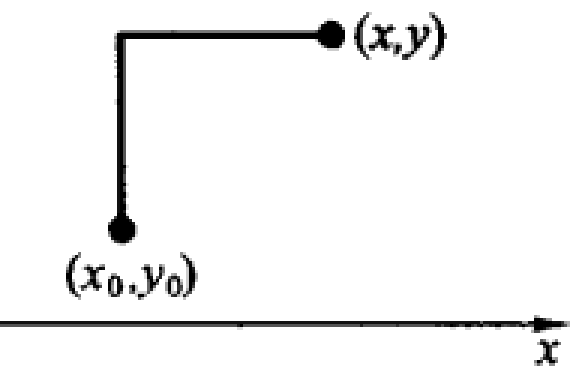
\includegraphics[width=\textwidth]{work/figures/fig22-21b}
\end{minipage}\caption{\relax}\label{fig:22-21}
\end{figure}
\[
u(x,y)=\int_{y_{0}}^{y}Q(x_{0},y)\mathrm{d}y+\int_{x_{0}}^{x}P(x,y)\mathrm{d}x+C,
\]
或
\[
u(x,y)=\int_{x_{0}}^{x}P(x,y_{0})\mathrm{d}x+\int_{y_{0}}^{y}Q(x,y)\mathrm{d}y+C.
\]
其中 $C$ 为常数．这是两个定积分之和，一般说来，我们是会计算的．

\begin{example}\label{ex:22-2-2}
求 $\left(\cos x+2x\sin y\right)\mathrm{d}x+\left(x^{2}\cos y\right)\mathrm{d}y$ 的原函数．
\end{example}

\begin{proof}[解]
设 $P(x,y)=\cos x+2x\sin y$，$Q(x,y)=x^{2}\cos y$．易见 $P$、$Q$ 在全平面上有连续的偏导数，且
\[
\frac{\partial P}{\partial y}=2x\cos y=\frac{\partial Q}{\partial x}.
\]
因此在平面上的任意光滑曲线 $AB$ 的积分
\[
\int_{\widehat{AB}}\left(\cos x+2x\sin y\right)\mathrm{d}x+\left(x^{2}\cos y\right)\mathrm{d}y
\]
只与起点 $A$ 和终点 $B$ 有关，而与路径的选择无关．取 $A=(0,0)$，$B=(x,y)$，则有
\[
\begin{aligned}
u(x,y)&=\int_{0}^{x}P(x,0)\mathrm{d}x+\int_{0}^{y}Q(x,y)\mathrm{d}y+C\\
&=\int_{0}^{x}\cos x\,\mathrm{d}x+\int_{0}^{y}x^{2}\cos y\,\mathrm{d}y+C\\
&=\sin x+x^{2}\sin y+C,
\end{aligned}
\]
这便是所要求的原函数．

当然，在简单的情形下我们可以通过观察直接凑微分，例如
\[
\begin{aligned}
&\left(\cos x+2x\sin y\right)\mathrm{d}x+\left(x^{2}\cos y\right)\mathrm{d}y\\
=&\cos x\,\mathrm{d}x+\left(2x\sin y\,\mathrm{d}x+x^{2}\cos y\,\mathrm{d}y\right)\\
=&\mathrm{d}\sin x+\mathrm{d}\left(x^{2}\sin y\right)\\
=&\mathrm{d}\left(\sin x+x^{2}\sin y\right),
\end{aligned}
\]
故 $u(x,y)=\sin x+x^{2}\sin y+C$．这样也得到同样的结果．
\end{proof}

定理~\ref{thm:22-4} 可以推广到三维的情形．

\begin{theorem}\label{thm:22-5}
设 $V$ 是空间的单连通区域，函数 $P$、$Q$、$R$ 在 $V$ 上有连续偏导数，则下列四断言等价：
\begin{enumerate}[label=（\arabic*）]
\item 沿 $V$ 内任一逐段光滑闭曲线 $L$，有 $\displaystyle\oint_{L}P\mathrm{d}x+Q\mathrm{d}y+R\mathrm{d}z=0$；
\item 对 $V$ 内任一逐段光滑曲线 $L$，曲线积分 $\displaystyle\int_{L}P\mathrm{d}x+Q\mathrm{d}y+R\mathrm{d}z$ 与路径无关，只与 $L$ 的起点与终点有关；
\item 微分式 $P\mathrm{d}x+Q\mathrm{d}y+R\mathrm{d}z$ 在 $V$ 内是某函数 $u(x,y,z)$ 的全微分，即 $\mathrm{d}u=P\mathrm{d}x+Q\mathrm{d}y+R\mathrm{d}z$；
\item 在 $V$ 内每一点有 $\dfrac{\partial P}{\partial y}=\dfrac{\partial Q}{\partial x}$，$\dfrac{\partial Q}{\partial z}=\dfrac{\partial R}{\partial y}$，$\dfrac{\partial R}{\partial x}=\dfrac{\partial P}{\partial z}$．
\end{enumerate}
\end{theorem}

定理~\ref{thm:22-5} 的证明可类似于定理~\ref{thm:22-4} 进行，困难在（4）$\Rightarrow$（1）时，如何用斯托克斯公式，我们不在此详述了．

断言（4）也可写为：在 $V$ 内每一点有
\[
\begin{vmatrix}\bm{i}&\bm{j}&\bm{k}\\[3pt]\dfrac{\partial}{\partial x}&\dfrac{\partial}{\partial y}&\dfrac{\partial}{\partial z}\\[3pt] P&Q&R\end{vmatrix}=\bm{0}.
\]

\begin{xiti}
\item 验证下列积分与路径无关，并求它们的值：
\begin{ziti}
\item $\displaystyle\int_{(0,0)}^{(1,1)}(x-y)(\mathrm{d}x-\mathrm{d}y)$；
\item $\displaystyle\int_{(2,1)}^{(1,2)}\frac{y\mathrm{d}x-x\mathrm{d}y}{x^{2}}$ 沿在右半平面的路径；
\item $\displaystyle\int_{(1,0)}^{(6,8)}\frac{x\mathrm{d}x+y\mathrm{d}y}{x^{2}+y^{2}}$ 沿不通过原点的路径；
\item $\displaystyle\int_{(0,0)}^{(a,b)}f(x+y)(\mathrm{d}x+\mathrm{d}y)$，式中 $f(u)$ 是连续函数；
\item $\displaystyle\int_{(2,1)}^{(1,2)}\varphi(x)\mathrm{d}x+\psi(y)\mathrm{d}y$，其中 $\varphi$，$\psi$ 为连续函数；
\item $\displaystyle\int_{(1,2,3)}^{(6,1,1)}yz\mathrm{d}x+xz\mathrm{d}y+xy\mathrm{d}z$；
\item $\displaystyle\int_{(1,1,1)}^{(2,3,-4)}x\,\mathrm{d}x+y^{2}\,\mathrm{d}y-z^{3}\,\mathrm{d}z$；
\item $\displaystyle\int_{(x_{1},y_{1},z_{1})}^{(x_{2},y_{2},z_{2})}\frac{x\mathrm{d}x+y\mathrm{d}y+z\mathrm{d}z}{\sqrt{x^{2}+y^{2}+z^{2}}}$，其中 $(x_{1},y_{1},z_{1})$，$(x_{2},y_{2},z_{2})$ 在球面 $x^{2}+y^{2}+z^{2}=a^{2}$ 上．
\end{ziti}
\item 求下列全微分的原函数：
\begin{ziti}
\item $\left(x^{2}+2xy-y^{2}\right)\mathrm{d}x+\left(x^{2}-2xy-y^{2}\right)\mathrm{d}y$；
\item $\left(2x\cos y-y^{2}\sin x\right)\mathrm{d}x+\left(2y\cos x-x^{2}\sin y\right)\mathrm{d}y$；
\item $\dfrac{a}{z}\mathrm{d}x+\dfrac{b}{z}\mathrm{d}y+\dfrac{-by-ax}{z^{2}}\mathrm{d}z$；
\item $\left(x^{2}-2yz\right)\mathrm{d}x+\left(y^{2}-2xz\right)\mathrm{d}y+\left(z^{2}-2xy\right)\mathrm{d}z$；
\item $\left(\mathrm{e}^{x}\sin y+2xy^{2}\right)\mathrm{d}x+\left(\mathrm{e}^{x}\cos y+2x^{2}y\right)\mathrm{d}y$；
\item $\left[\dfrac{x}{\left(x^{2}-y^{2}\right)^{2}}-\dfrac{1}{x}+2x^{2}\right]\mathrm{d}x+\left[\dfrac{1}{y}-\dfrac{y}{\left(x^{2}-y^{2}\right)^{2}}+3y^{3}\right]\mathrm{d}y+5z^{3}\mathrm{d}z$.
\end{ziti}
\item 函数 $F(x,y)$ 应满足什么条件才能使微分式
\[
F(x,y)(x\mathrm{d}x+y\mathrm{d}y)
\]
是全微分．
\item 验证
\[
P\mathrm{d}x+Q\mathrm{d}y=\frac{1}{2}\frac{x\mathrm{d}y-y\mathrm{d}x}{Ax^{2}+2Bxy+Cy^{2}}
\]
适合条件 $\dfrac{\partial P}{\partial y}=\dfrac{\partial Q}{\partial x}$，其中 $A$，$B$，$C$ 为常数，$AC-B^{2}>0$．求奇点 $(0,0)$ 的循环常数．
\item 求 $I=\displaystyle\oint_{L}\frac{x\,\mathrm{d}x+y\,\mathrm{d}y}{x^{2}+y^{2}}$，其中 $L$ 是不经过原点的简单闭曲线，取正向．设 $L$ 围成的区域为 $D$．（1）$D$ 不包含原点；（2）$D$ 包含原点在其内部．
\item 求
\[
I=\oint_{L}\left[\frac{y}{(x-2)^{2}+y^{2}}+\frac{y}{(x+2)^{2}+y^{2}}\right]\mathrm{d}x+\left[\frac{2-x}{(2-x)^{2}+y^{2}}+\frac{-(2+x)}{(2+x)^{2}+y^{2}}\right]\mathrm{d}y,
\]
其中 $L$ 是不经过 $(-2,0)$ 和 $(2,0)$ 点的简单闭曲线．
\item 设 $u(x,y)$ 在平面单连通区域 $D$ 上有二阶连续偏导数，证明 $u(x,y)$ 在 $D$ 内有 $\dfrac{\partial^{2}u}{\partial x^{2}}+\dfrac{\partial^{2}u}{\partial y^{2}}=0$ 的充要条件是对 $D$ 内任一简单光滑闭曲线 $L$，都有
\[
\oint_{L}\frac{\partial u}{\partial n}\mathrm{d}s=0,
\]
其中 $\dfrac{\partial u}{\partial n}$ 为 $L$ 沿外法线方向的方向导数．
\item 计算积分
\[
I=\int_{L}\frac{(x+y)\mathrm{d}x-(x-y)\mathrm{d}y}{x^{2}+y^{2}},
\]
其中 $L$ 是从点 $A(-1,0)$ 到 $B(1,0)$ 的一条不通过原点的光滑曲线，它的方程是 $y=f(x)$（$-1\leqslant x\leqslant 1$）．
\item 计算积分
\[
I=\int_{L}x\ln(x^{2}+y^{2}-1)\mathrm{d}x+y\ln(x^{2}+y^{2}-1)\mathrm{d}y,
\]
其中 $L$ 是被积函数的定义域内从点 $(2,0)$ 至 $(0,2)$ 的逐段光滑曲线．
\end{xiti}

\section{场论初步}

在第二十一章 §2 中，我们介绍了速度向量场的概念．一般地，向量场不仅仅是速度场，还可以有磁场、力场等等．场也不仅仅有向量场，还有数量场，例如温度场．若对空间某一区域 $V$ 中的每一点 $(x,y,z)$ 以及每一时刻 $t$，都对应一个数量 $u(x,y,z,t)$，则在 $V$ 上确定的是一个数量场 $u$；若对应的是一个向量 $\bm{F}(x,y,z,t)$，则在 $V$ 上确定的是向量场 $\bm{F}$．数量场和向量场统称为场．当场不依赖于时间 $t$ 时，称为定常场．

本节讨论定常场，介绍与场论有关的若干概念，并给出高斯公式等的场论解释．

\subsection{梯度场}

设 $u(x,y,z)$ 是在空间某区域 $V$ 上给定的一个数量场，函数 $u(x,y,z)$ 在 $V$ 上存在连续偏导数．这时 $V$ 中的每一点 $(x,y,z)$ 都对应一个向量
\[
\left(\frac{\partial u}{\partial x},\frac{\partial u}{\partial y},\frac{\partial u}{\partial z}\right),
\]
我们称它为函数 $u(x,y,z)$ 在 $(x,y,z)$ 的\emph{梯度}（gradient），记为 $\mathrm{grad}\,u$（$\mathrm{grad}$ 是 gradient 的缩写）．当 $(x,y,z)$ 取遍 $V$ 的所有点时，$\mathrm{grad}\,u$ 便定义了 $V$ 上的一个向量场，我们称它为数量场 $u(x,y,z)$ 的\emph{梯度场}，称 $u(x,y,z)$ 为梯度场的\emph{势函数}．记
\[
\nabla=\left(\frac{\partial}{\partial x},\frac{\partial}{\partial y},\frac{\partial}{\partial z}\right),
\]
称 $\nabla$ 为哈密顿（Hamilton，W．R．，$1805$—$1865$）算子．把 $\nabla$ 看作向量，则梯度就可以形式地写成向量 $\nabla$ 与数量 $u$ 的数量积，即
\[
\mathrm{grad}\,u=\nabla u=\left(\frac{\partial}{\partial x},\frac{\partial}{\partial y},\frac{\partial}{\partial z}\right)u=\left(\frac{\partial u}{\partial x},\frac{\partial u}{\partial y},\frac{\partial u}{\partial z}\right).
\]
利用梯度，函数 $u(x,y,z)$ 沿 $\bm{l}=(\cos\alpha,\cos\beta,\cos\gamma)$ 的方向导数可表为
\[
\begin{aligned}
\frac{\partial u}{\partial l}&=\frac{\partial u}{\partial x}\cos\alpha+\frac{\partial u}{\partial y}\cos\beta+\frac{\partial u}{\partial z}\cos\gamma\\
&=\mathrm{grad}\,u\cdot\bm{l}=|\mathrm{grad}\,u|\cos\theta,
\end{aligned}
\]
其中 $\mathrm{grad}\,u\cdot\bm{l}$ 是向量的内积，而 $\theta$ 是 $\bm{l}$ 与梯度 $\mathrm{grad}\,u$ 之间的夹角．在给定点 $(x,y,z)$，梯度是唯一确定的，上式表明，$u$ 沿 $\bm{l}$ 的方向导数，正是梯度向量在 $\bm{l}$ 的投影．因此，当 $\theta=0$，即 $\bm{l}$ 与 $\mathrm{grad}\,u$ 方向相同时，$\dfrac{\partial u}{\partial l}$ 达到最大值 $|\mathrm{grad}\,u|$，这表明沿梯度方向函数 $u$ 的值增长最快；当 $\theta=\pi$，即 $\bm{l}$ 与 $\mathrm{grad}\,u$ 方向相反时，$\dfrac{\partial u}{\partial l}$ 达到最小值 $-|\mathrm{grad}\,u|$，它表明沿梯度的反方向函数 $u$ 的值下降最快；$\theta=\dfrac{\pi}{2}$，即 $\bm{l}$ 与 $\mathrm{grad}\,u$ 垂直时，$\dfrac{\partial u}{\partial l}=0$，它表明与梯度垂直的方向函数 $u$ 是稳定的．

一个向量，如果给定了它的方向和大小，则这个向量便唯一确定了．因此，根据上面的讨论，我们可以给出梯度的另一个等价定义：数量场 $u$ 在任一点的梯度是一个向量，它的方向是数量函数 $u$ 在这点增长最快的方向，而它的大小则等于 $u$ 在这点沿该方向的方向导数．

梯度的两个定义各有特点，第一个定义是定量的，便于计算，但容易引起错觉，似乎梯度场是与坐标系的选择有关的．而第二个定义是定性的，它给我们很直观的物理意义．数量场在任一点沿任一方向的变化率是与坐标系的选取无关的，由此可知梯度与坐标系的选取无关．

满足
\[
u(x,y,z)\equiv c
\]
的点 $(x,y,z)$ 构成的曲面称为数量场 $u$ 的等值面．在等值面上数量场 $u$ 的值不变．注意到曲面 $u(x,y,z)=c$ 在 $(x,y,z)$ 的法向量为 $\left(\dfrac{\partial u}{\partial x},\dfrac{\partial u}{\partial y},\dfrac{\partial u}{\partial z}\right)$，它正好是数量场在 $(x,y,z)$ 的梯度．这就说明了数量场在一点的梯度垂直于过该点的等值面，指向数量场增加的方向，其大小等于 $u$ 沿此方向的方向导数．

\begin{example}\label{ex:22-3-1}
设 $u(x,y,z)=x^{2}+y^{2}+z^{2}$，函数在任一点的梯度为
\[
\mathrm{grad}\,u=(2x,2y,2z)=2\bm{r},
\]
即梯度的方向就是矢径 $\bm{r}=(x,y,z)$ 的方向．梯度的大小为
\[
|\mathrm{grad}\,u|=2|\bm{r}|=2\sqrt{x^{2}+y^{2}+z^{2}}.
\]
从几何上看，函数 $u$ 的等值面是一族球面，球面的法向量平行于 $\bm{r}$，沿 $\bm{r}$ 方向函数 $u$ 增长最快，因此这个方向就是梯度方向．而沿 $\bm{r}$ 的反方向，函数 $u$ 下降最快．
\end{example}

\begin{example}\label{ex:22-3-2}
设质量为 $m$ 的质点位于原点，质量为 $1$ 的质点位于 $M(x,y,z)$，记 $OM=r=\sqrt{x^{2}+y^{2}+z^{2}}$，求 $u=\dfrac{m}{r}$ 的梯度．
\end{example}

\begin{figure}[htbp]
\centering
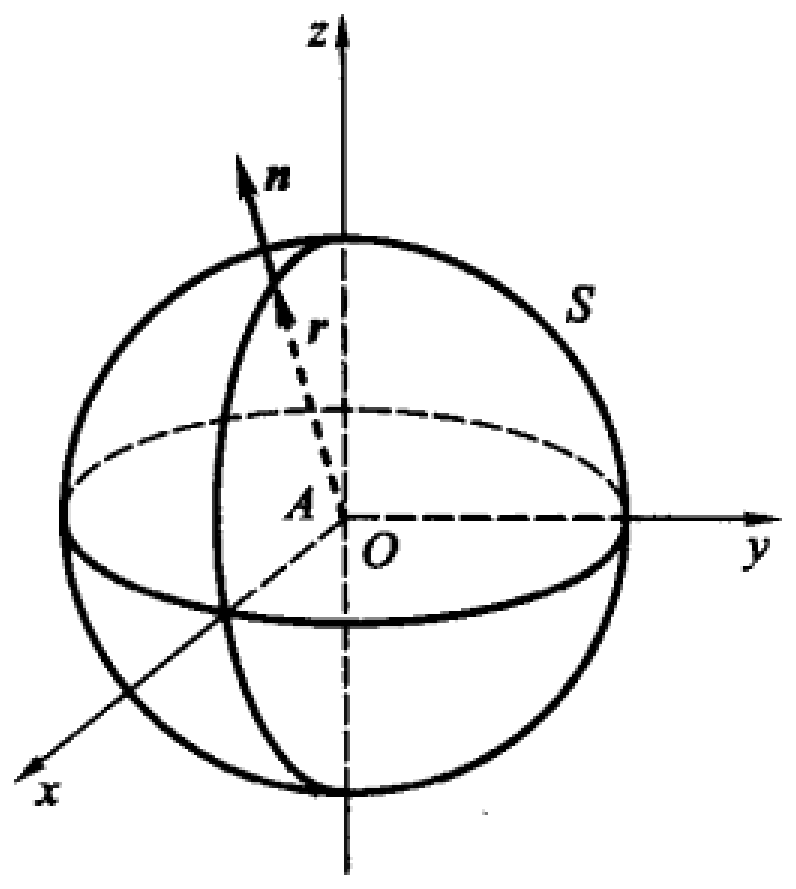
\includegraphics[width=0.28\textwidth]{work/figures/fig22-22}\caption{\relax}\label{fig:22-22}
\end{figure}

\begin{proof}[解]
\[
\frac{\partial u}{\partial x}=-\frac{m}{r^{2}}\frac{\partial r}{\partial x}=-\frac{m}{r^{2}}\frac{x}{r}.
\]
由 $x$，$y$，$z$ 的对称性得
\[
\mathrm{grad}\,u=-\frac{m}{r^{2}}\left(\frac{x}{r},\frac{y}{r},\frac{z}{r}\right)=-\frac{m}{r^{2}}\bm{r}_{0}.
\]
这里 $\bm{r}_{0}$ 是 $\bm{r}$ 方向的单位向量．上式的右端在数量上的大小恰好是两质点间的引力，方向指向原点．它表明引力场是数量场 $\dfrac{m}{r}$ 的梯度场．因此 $\dfrac{m}{r}$ 常被称为引力势．
\end{proof}

\subsection{散度场}

设 $\bm{F}(x,y,z)=\left(P(x,y,z),Q(x,y,z),R(x,y,z)\right)$ 是展布在空间某区域 $V$ 上的向量场，函数 $P$，$Q$，$R$ 在 $V$ 上存在对各变元的连续偏导数，则在 $V$ 上每一点 $(x,y,z)$，数量函数
\[
\frac{\partial P}{\partial x}+\frac{\partial Q}{\partial y}+\frac{\partial R}{\partial z}
\]
称为向量场 $\bm{F}(x,y,z)$ 在 $(x,y,z)$ 处的\emph{散度}，记作
\[
\mathrm{div}\,\bm{F}(x,y,z)=\frac{\partial P}{\partial x}+\frac{\partial Q}{\partial y}+\frac{\partial R}{\partial z}
\]
（$\mathrm{div}$ 是 divergence 的缩写），当 $(x,y,z)$ 取遍 $V$ 的点时，散度也就构成了 $V$ 的一个数量场——散度场 $\mathrm{div}\,\bm{F}(x,y,z)$．

散度场 $\mathrm{div}\,\bm{F}(x,y,z)$ 是由向量场 $\bm{F}(x,y,z)$ 产生的数量场，沿用前面提到的哈密顿算子，则散度又可表为向量 $\nabla$ 与向量 $\bm{F}$ 的内积，即
\[
\mathrm{div}\,\bm{F}(x,y,z)=\nabla\cdot\bm{F}.
\]
利用散度，高斯公式
\[
\begin{aligned}
&\iiint_{V}\left(\frac{\partial P}{\partial x}+\frac{\partial Q}{\partial y}+\frac{\partial R}{\partial z}\right)\mathrm{d}x\mathrm{d}y\mathrm{d}z\\
=&\oiint_{S}\left(P\mathrm{d}y\mathrm{d}z+Q\mathrm{d}z\mathrm{d}x+R\mathrm{d}x\mathrm{d}y\right)
\end{aligned}
\]
可以表示为向量形式：
\[
\iiint_{V}\mathrm{div}\,\bm{F}(x,y,z)\mathrm{d}x\mathrm{d}y\mathrm{d}z=\oiint_{S}\bm{F}\cdot\mathrm{d}\bm{S}.
\]
下面我们根据高斯公式，给出散度的另一种解释．对 $V$ 中任意点 $M_{0}(x_{0},y_{0},z_{0})$，取 $V_{1}$ 为包含 $M_{0}$ 的小区域，$S$ 是其边界曲面（取外侧），则上式仍成立．对上式左端的三重积分用中值定理，知存在 $M^{*}\in V_{1}$，使得
\[
\mathrm{div}\,\bm{F}(M^{*})\left|V_{1}\right|=\oiint_{S}\bm{F}\cdot\mathrm{d}\bm{S}.
\]
令 $V_{1}$ 收缩到 $M_{0}$，即对 $M_{0}\in V_{1}$，令 $d(V_{1})\to 0$，此时 $M^{*}\to M_{0}$，因此
\[
\mathrm{div}\,\bm{F}(M_{0})=\lim_{\substack{d(V_{1})\to 0\\ M_{0}\in V_{1}}}\mathrm{div}\,\bm{F}(M^{*})=\lim_{\substack{d(V_{1})\to 0\\ M_{0}\in V_{1}}}\frac{\displaystyle\oiint_{S}\bm{F}\cdot\mathrm{d}\bm{S}}{\left|V_{1}\right|}.
\]
上式有一种力学的解释．如果 $\bm{F}$ 是流体的流速场，则第二十一章 §2 的讨论告诉我们，$\displaystyle\oiint_{S}\bm{F}\cdot\mathrm{d}\bm{S}$ 是流速为 $\bm{F}$ 的流体在单位时间内流过曲面 $S$ 的流量，而 $\dfrac{1}{\left|V_{1}\right|}\displaystyle\oiint_{S}\bm{F}\cdot\mathrm{d}\bm{S}$ 便是 $V_{1}$ 内的平均流量，即在平均的意义下，单位体积流出的流量．因此其极限 $\mathrm{div}\,\bm{F}(M_{0})$ 就是流体在 $M_{0}$ 点的单位体积的流量，也就是流体速度场 $\bm{F}$ 在 $M_{0}$ 点的流量密度．显然，这个物理量是不依赖于坐标系的，这就说明了散度与坐标系的选取无关．

注意到高斯公式中表示流量的曲面积分是取外侧的，故若 $\mathrm{div}\,\bm{F}(M_{0})>0$，它表示在单位时间内有流体流出这一点，这时称 $M_{0}$ 点为\emph{源}（源泉）；若 $\mathrm{div}\,\bm{F}(M_{0})<0$，它表示在单位时间内有流体流入这一点，这时称 $M_{0}$ 点为\emph{汇}（渗入点、吸收点）．

有了散度的概念后，又可以反过来，给出高斯公式
\[
\iiint_{V}(\mathrm{div}\,\bm{F})\mathrm{d}V=\oiint_{S}\bm{F}\cdot\mathrm{d}\bm{S}
\]
的力学解释．这就是单位时间流出闭曲面 $S$ 的流量，等于区域内每一点渗出率（流量密度 $\mathrm{div}\,\bm{F}$ 乘体积元 $\mathrm{d}V$）的总和．这和我们的常识是吻合的．当向量场 $\bm{F}$ 在 $V$ 中每一点的散度皆为零时，即
\[
\mathrm{div}\,\bm{F}(M)\equiv 0,
\]
则 $V$ 内每一点既不是源也不是汇，这时称 $\bm{F}$ 为\emph{无源场}．

对无源场，有
\[
\oiint_{S}\bm{F}\cdot\mathrm{d}\bm{S}=0.
\]
它说明，流过 $V$ 的流量的代数和为 $0$，即流入 $V$ 的流量与流出 $V$ 的流量相互抵消，这与``无源''的直观是完全符合的．

\begin{example}\label{ex:22-3-3}
例~\ref{ex:22-3-2} 中由函数 $\dfrac{m}{r}$ 产生的梯度场为
\[
\mathrm{grad}\,u=-\frac{m}{r^{2}}\left(\frac{x}{r},\frac{y}{r},\frac{z}{r}\right),
\]
求 $\mathrm{grad}\,u$ 产生的散度场．
\end{example}

\begin{proof}[解]
记 $P(x,y,z)=-\dfrac{m}{r^{3}}x$，则
\[
\frac{\partial P}{\partial x}=-\frac{m}{r^{3}}+\frac{3mx}{r^{4}}\frac{\partial r}{\partial x}=-\frac{m}{r^{3}}+\frac{3mx}{r^{4}}\frac{x}{r}.
\]
由 $x$，$y$，$z$ 的对称性即知
\[
\mathrm{div}\,\mathrm{grad}\,u=-\frac{3m}{r^{3}}+\frac{3mx^{2}}{r^{5}}+\frac{3my^{2}}{r^{5}}+\frac{3mz^{2}}{r^{5}}=0.
\]
此例表明引力场的散度场是无源场．
\end{proof}

\subsection{旋度场}

设 $\bm{F}(x,y,z)=\left(P(x,y,z),Q(x,y,z),R(x,y,z)\right)$ 是展布在空间某区域 $V$ 上的向量场，函数 $P$，$Q$，$R$ 在 $V$ 上存在对各变元的连续偏导数，则在 $V$ 上每一点 $(x,y,z)$，向量函数
\[
\left(\frac{\partial R}{\partial y}-\frac{\partial Q}{\partial z},\ \frac{\partial P}{\partial z}-\frac{\partial R}{\partial x},\ \frac{\partial Q}{\partial x}-\frac{\partial P}{\partial y}\right)
\]
称为向量场 $\bm{F}(x,y,z)$ 在 $(x,y,z)$ 处的\emph{旋度}，记作 $\mathrm{rot}\,\bm{F}(x,y,z)$（$\mathrm{rot}$ 是 rotation 的缩写）．当 $(x,y,z)$ 取遍区域 $V$ 的点时，$\mathrm{rot}\,\bm{F}(x,y,z)$ 便定义了 $V$ 的一个向量场，称为 $\bm{F}$ 的\emph{旋度场}．旋度场 $\mathrm{rot}\,\bm{F}(x,y,z)$ 是由向量场 $\bm{F}(x,y,z)$ 产生的向量场．

为便于记忆，常把旋度表为
\[
\mathrm{rot}\,\bm{F}(x,y,z)=\begin{vmatrix}\bm{i}&\bm{j}&\bm{k}\\[3pt]\dfrac{\partial}{\partial x}&\dfrac{\partial}{\partial y}&\dfrac{\partial}{\partial z}\\[3pt] P&Q&R\end{vmatrix}=\nabla\times\bm{F},
\]
即旋度是向量 $\nabla$ 与向量 $\bm{F}$ 的外积．

利用旋度，斯托克斯公式可以表示为向量形式：
\[
\iint_{S}\mathrm{rot}\,\bm{F}\cdot\mathrm{d}\bm{S}=\oint_{L}\bm{F}\cdot\mathrm{d}\bm{s}
\]
或
\[
\iint_{S}\mathrm{rot}\,\bm{F}\cdot\bm{n}\,\mathrm{d}S=\oint_{L}\bm{F}\cdot\mathrm{d}\bm{s},
\]
其中 $\bm{n}$ 为曲面 $S$ 在规定侧的单位法向量．上式中，右边的积分
\[
\oint_{L}\bm{F}\cdot\mathrm{d}\bm{s}=\oint_{L}P\mathrm{d}x+Q\mathrm{d}y+R\mathrm{d}z
\]
称为向量场 $\bm{F}$ 沿闭曲线 $L$ 的\emph{环流量}，它反映了向量场 $\bm{F}$ 沿 $L$ 的旋转强弱程度．

与散度一样，旋度是与坐标的选取无关的．事实上，在 $M_{0}$ 点选定一个单位方向 $\bm{n}$，过 $M_{0}$ 点作平面 $\pi$ 垂直于 $\bm{n}$，在 $\pi$ 上围绕 $M_{0}$ 点作一简单封闭曲线 $L$，其方向和 $\bm{n}$ 的方向构成右手法则，$L$ 所围平面区域为 $D$，则由斯托克斯公式，有
\[
\iint_{D}\mathrm{rot}\,\bm{F}\cdot\bm{n}\,\mathrm{d}S=\oint_{L}\bm{F}\cdot\mathrm{d}\bm{s}.
\]
由二重积分中值定理，存在 $M^{*}\in D$，使得
\[
\mathrm{rot}\,\bm{F}(M^{*})\cdot\bm{n}\,|D|=\oint_{L}\bm{F}\cdot\mathrm{d}\bm{s}.
\]
令 $D$ 收缩到点 $M_{0}$，记为 $D\to M_{0}$，此时有 $M^{*}\to M_{0}$，故
\[
\mathrm{rot}\,\bm{F}(M_{0})\cdot\bm{n}=\lim_{D\to M_{0}}\frac{\displaystyle\oint_{L}\bm{F}\cdot\mathrm{d}\bm{s}}{|D|}.
\]
这公式说明，$\bm{F}$ 在 $M_{0}$ 的旋度在 $\bm{n}$ 方向的投影 $\mathrm{rot}\,\bm{F}(M_{0})\cdot\bm{n}$ 等于在 $M_{0}$ 的单位面积的环流量，显然这个物理量是不依赖于坐标系的．只要知道向量 $\mathrm{rot}\,\bm{F}(M_{0})$ 在任意方向 $\bm{n}$ 上的投影，便完全确定了向量 $\mathrm{rot}\,\bm{F}(M_{0})$ 的本身．因此旋度与坐标系的选取无关．

如果在 $V$ 中每一点 $M$，有 $\mathrm{rot}\,\bm{F}(M)\equiv 0$，则称 $\bm{F}$ 为\emph{无旋场}．

为了进一步说明旋度的物理意义，我们来看刚体以固定的角速度 $\bm{\omega}$ 绕某过原点的轴旋转．这时角速度 $\bm{\omega}$ 的方向平行于旋转轴，线速度 $\bm{v}$ 与 $\bm{\omega}$ 构成右手法则，且
\[
\begin{aligned}
\bm{v}=\bm{\omega}\times\bm{r}&=\begin{vmatrix}\bm{i}&\bm{j}&\bm{k}\\ \omega_{x}&\omega_{y}&\omega_{z}\\ x&y&z\end{vmatrix}\\
&=\left(z\omega_{y}-y\omega_{z}\right)\bm{i}+\left(x\omega_{z}-z\omega_{x}\right)\bm{j}+\left(y\omega_{x}-x\omega_{y}\right)\bm{k}.
\end{aligned}
\]
\begin{figure}[htbp]
\centering
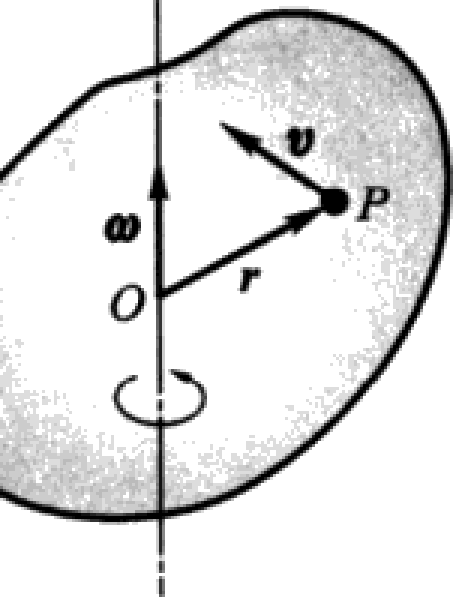
\includegraphics[width=0.22\textwidth]{work/figures/fig22-23}\caption{\relax}\label{fig:22-23}
\end{figure}
我们来计算速度场 $\bm{v}$ 的旋度，得
\[
\mathrm{rot}\,\bm{v}=\begin{vmatrix}\bm{i}&\bm{j}&\bm{k}\\[3pt]\dfrac{\partial}{\partial x}&\dfrac{\partial}{\partial y}&\dfrac{\partial}{\partial z}\\[3pt] z\omega_{y}-y\omega_{z}&x\omega_{z}-z\omega_{x}&y\omega_{x}-x\omega_{y}\end{vmatrix}=2\bm{\omega}.
\]
上式表明线速度 $\bm{v}$ 的旋度 $\mathrm{rot}\,\bm{v}$ 等于角速度 $\bm{\omega}$ 的二倍．当角速度 $\bm{\omega}\equiv 0$ 时，刚体无旋转，$\mathrm{rot}\,\bm{v}\equiv 0$．这说明向量场 $\bm{F}$ 的旋度 $\mathrm{rot}\,\bm{F}$ 反映了 $\bm{F}$ 在一点附近的旋转强弱的程度与方向．

\subsection{\texorpdfstring{梯度、散度、旋度等于零的充要条件}{梯度、散度、旋度等于零的充要条件}}

\begin{theorem}\label{thm:22-6}
设 $V$ 是空间某单连通区域，$u(x,y,z)$ 在 $V$ 内有连续偏导数，则在 $V$ 内，$\mathrm{grad}\,u\equiv 0$ 的充要条件是数量场 $u(x,y,z)$ 是常量场．
\end{theorem}

\begin{proof}
充分性显然成立，下证必要性．由 $\mathrm{grad}\,u=\bm{0}$，即
\[
\frac{\partial u}{\partial x}=\frac{\partial u}{\partial y}=\frac{\partial u}{\partial z}\equiv 0.
\]
设 $M_{1}$ 和 $M_{2}$ 是 $V$ 内任意两点，则在 $V$ 内任一从 $M_{1}$ 到 $M_{2}$ 的逐段光滑曲线 $L$，曲线积分
\[
\int_{L}\frac{\partial u}{\partial x}\mathrm{d}x+\frac{\partial u}{\partial y}\mathrm{d}y+\frac{\partial u}{\partial z}\mathrm{d}z=\int_{L}\mathrm{d}u\equiv 0.
\]
而
\[
\int_{L}\mathrm{d}u=\int_{M_{1}}^{M_{2}}\mathrm{d}u=u(M_{2})-u(M_{1}),
\]
因此
\[
u(M_{1})\equiv u(M_{2}).
\]
由 $M_{1}$ 和 $M_{2}$ 的任意性即知 $u$ 是常量场．定理~\ref{thm:22-6} 证完．
\end{proof}

\begin{theorem}\label{thm:22-7}
设 $\Omega$ 是空间单连通区域，$\bm{F}=(P,Q,R)$ 是展布在 $\Omega$ 上的向量场，$P$，$Q$，$R$ 在 $\Omega$ 内有连续的偏导数，则在 $\Omega$ 内 $\mathrm{div}\,\bm{F}(x,y,z)\equiv 0$ 的充要条件是对 $\Omega$ 内任一分片光滑的封闭曲面 $S$，有 $\displaystyle\oiint\bm{F}\cdot\mathrm{d}\bm{S}=0$．
\end{theorem}

\begin{proof}
必要性．对 $\Omega$ 内任一分片光滑封闭曲面 $S$，由高斯公式立得
\[
\oiint_{S}\bm{F}\cdot\mathrm{d}\bm{S}=\iiint_{V}\mathrm{div}\,\bm{F}(M)\mathrm{d}V=0.
\]
充分性，对任意 $M_{0}\in\Omega$，取 $V$ 为以 $M_{0}$ 为中心半径为 $r$ 的球体，$S$ 是它的边界球面，则由散度的公式知
\[
\mathrm{div}\,\bm{F}(M_{0})=\lim_{V\to M_{0}}\frac{\displaystyle\oiint_{S}\bm{F}\cdot\mathrm{d}\bm{S}}{|V|}=0.
\]
定理~\ref{thm:22-7} 证完．
\end{proof}

满足定理~\ref{thm:22-7} 中必要条件的场 $\bm{F}$ 称为\emph{管量场}，因此定理~\ref{thm:22-7} 又可叙述为 $\bm{F}$ 是无源场的充要条件为 $\bm{F}$ 是管量场．

在向量场 $\bm{F}=(P,Q,R)$ 中，如果曲线上每一点的切线平行于该点的场向量 $\bm{F}$，即
\[
\frac{\mathrm{d}x}{P}=\frac{\mathrm{d}y}{Q}=\frac{\mathrm{d}z}{R},
\]
则称曲线 $L$ 为向量场的\emph{向量线}．由向量线围成的管状曲面称为\emph{向量管}．在向量管上任取两断面 $S_{1}$，$S_{2}$，以 $S_{3}$ 表示截出的管的侧表面，则 $S=S_{1}\cup S_{2}\cup S_{3}$ 是一封闭曲面，因为曲面 $S_{3}$ 的法向量垂直于 $\bm{F}$，因此
\[
\iint_{S_{3}}\bm{F}\cdot\mathrm{d}\bm{S}=\iint_{S_{3}}\bm{F}\cdot\bm{n}\,\mathrm{d}S=0,
\]
\begin{figure}[htbp]
\centering
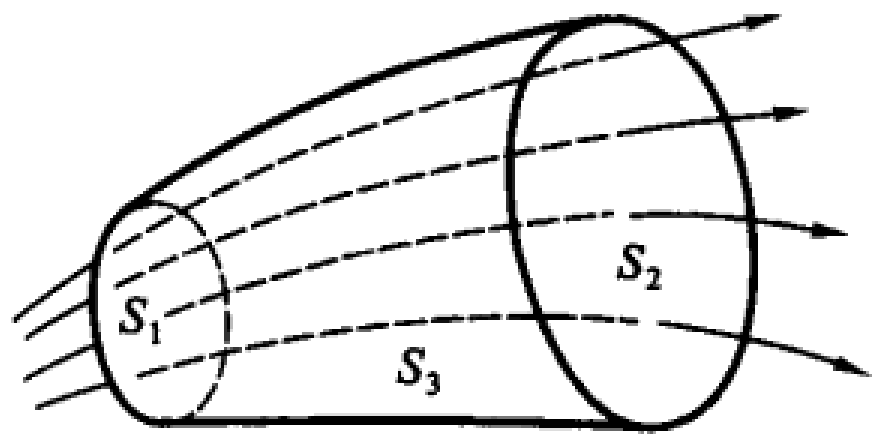
\includegraphics[width=0.32\textwidth]{work/figures/fig22-24}\caption{\relax}\label{fig:22-24}
\end{figure}
从而对 $S$ 的外侧，
\[
\oiint_{S}\bm{F}\cdot\mathrm{d}\bm{S}=0
\]
当且仅当
\[
\left(\iint_{S_{1}}+\iint_{S_{2}}\right)\bm{F}\cdot\mathrm{d}\bm{S}=0.
\]
即
\[
\iint_{S_{2}}\bm{F}\cdot\mathrm{d}\bm{S}=-\iint_{S_{1}}\bm{F}\cdot\mathrm{d}\bm{S}.
\]
可见管量场的物理意义是流体通过向量管的任意断面的流量相等．这也是管量场名称的由来．

最后我们讨论旋度等于零的充要条件．其实，它就是定理~\ref{thm:22-5} 中积分与路径无关的四个等价条件．

设 $V$ 是空间的单连通区域，$\bm{F}=(P,Q,R)$ 是展布在 $V$ 上的向量场，$P$，$Q$，$R$ 在 $V$ 内有连续偏导数，若对 $V$ 内任一逐段光滑封闭曲线 $L$，有
\[
\oint_{L}\bm{F}\cdot\mathrm{d}\bm{s}=0,
\]
则称 $\bm{F}$ 是\emph{有势场}．若对 $V$ 内任一逐段光滑曲线 $L$，有 $\displaystyle\int_{L}\bm{F}\cdot\mathrm{d}\bm{s}$ 与路径无关，则称 $\bm{F}$ 是\emph{保守场}．这样定理~\ref{thm:22-5} 又可叙述为：

\begin{theorem}\label{thm:22-8}
设 $V$ 是空间的单连通区域，$\bm{F}=(P,Q,R)$ 在 $V$ 内有连续偏导数，则下列四条件等价：
\begin{enumerate}[label=（\arabic*）]
\item $\bm{F}$ 是有势场；
\item $\bm{F}$ 是保守场；
\item $\bm{F}$ 是梯度场；
\item $\bm{F}$ 是无旋场．
\end{enumerate}
\end{theorem}

例~\ref{ex:22-3-3} 中已证
\[
\mathrm{div}\,\mathrm{grad}\left(\frac{m}{r}\right)=0.
\]
即 $\bm{F}=\mathrm{grad}\left(\dfrac{m}{r}\right)$ 是无源场，从而是管量场．又由 $\bm{F}$ 的定义知 $\bm{F}$ 是梯度场，这又等价于 $\bm{F}$ 是有势场、保守场和无旋场．

一个向量场 $\bm{F}$ 若同时是管量场和有势场，则称这个向量场为\emph{调和场}．这时存在势函数 $u$，满足
\[
\bm{F}=\mathrm{grad}\,u,\qquad\mathrm{div}\,\mathrm{grad}\,u=0.
\]
它等价于
\[
\frac{\partial^{2}u}{\partial x^{2}}+\frac{\partial^{2}u}{\partial y^{2}}+\frac{\partial^{2}u}{\partial z^{2}}=0.
\]
这时函数 $u$ 称为\emph{调和函数}．

例~\ref{ex:22-3-3} 表明 $\dfrac{m}{r}$ 是调和函数．

根据上面的讨论易知，对任意向量场 $\bm{A}$，有

（1）$\mathrm{div}\,\mathrm{rot}\,\bm{A}=\bm{0}$；

（2）$\mathrm{rot}\,\mathrm{grad}\,u=\bm{0}$．

我们把证明留给读者．

\begin{xiti}
\item 求 $u=x^{2}+2y^{2}+3z^{2}+2xy-4x+2y-4z$ 在点 $O(0,0,0)$，$A(1,1,1)$，$B(-1,-1,-1)$ 的梯度，并求梯度为零的点．
\item 计算下列向量场 $\bm{F}$ 的散度和旋度：
\begin{ziti}
\item $\bm{F}=(y^{2}+z^{2},\,z^{2}+x^{2},\,x^{2}+y^{2})$；
\item $\bm{F}=(x^{2}yz,\,xy^{2}z,\,xyz^{2})$；
\item $\bm{F}=\left(\dfrac{x}{yz},\,\dfrac{y}{zx},\,\dfrac{z}{xy}\right)$．
\end{ziti}
\item 证明 $\bm{F}=(yz(2x+y+z),\,xz(x+2y+z),\,xy(x+y+2z))$ 是有势场并求势函数．
\item 设 $P=x^{2}+5\lambda y+3yz$，$Q=5x+3\lambda xz-2$，$R=(\lambda+2)xy-4z$．
\begin{ziti}
\item 计算 $\displaystyle\int_{L}P\mathrm{d}x+Q\mathrm{d}y+R\mathrm{d}z$，其中 $L$ 是螺旋线 $x=a\cos t$，$y=a\sin t$，$z=ct$（$0\leqslant t\leqslant 2\pi$）；
\item 设 $\bm{F}=(P,Q,R)$，求 $\mathrm{rot}\,\bm{F}$；
\item 在什么条件下 $\bm{F}$ 为有势场，并求势函数．
\end{ziti}
\item 设 $\varphi$ 为可微函数，$\bm{r}=(x,y,z)$，$r=|\bm{r}|$，求 $\mathrm{grad}\,\varphi(r)$，$\mathrm{div}\,(\varphi(r)\bm{r})$，$\mathrm{rot}\,(\varphi(r)\bm{r})$．
\item 求向量场 $\bm{F}=(-y,x,z)$ 沿曲线 $L$ 的环流量：
\begin{ziti}
\item $L$ 为 $Oxy$ 平面上的圆周 $x^{2}+y^{2}=1$，$z=0$，逆时针方向；
\item $L$ 为 $Oxy$ 平面上的圆周 $(x-2)^{2}+y^{2}=R^{2}$，$z=0$，逆时针方向；
\item $L$ 为 $Oxy$ 平面上任一逐段光滑简单闭曲线，它围成的平面区域 $D$ 的面积为 $S$．证明 $\bm{F}$ 沿 $L$ 的环流量为 $2S$；
\item 设有一平面 $\pi$：$ax+by+cz=d$（$c\neq 0$），取 $\pi$ 为上侧，$\pi$ 上有一逐段光滑简单闭曲线 $L$，其方向关于 $\pi$ 为正向．$L$ 围成的平面区域的面积为 $S$，问 $\bm{F}$ 沿 $L$ 的环流量是什么？
\end{ziti}
\item 求向量场 $\bm{F}=\mathrm{grad}\left(\arctan\dfrac{y}{x}\right)$ 沿曲线 $L$ 的环流量：（1）$L$ 不环绕 $z$ 轴；（2）$L$ 环绕 $z$ 轴一圈；（3）$L$ 环绕 $z$ 轴 $n$ 圈．
\item 设向量场 $\bm{F}=(P,Q,R)$ 在除原点 $(0,0,0)$ 外有连续的偏导数，在球面 $x^{2}+y^{2}+z^{2}=t^{2}$ 上 $\bm{F}$ 的长度保持一固定值，$\bm{F}$ 的方向与矢径 $\bm{r}=(x,y,z)$ 相同，而且 $\bm{F}$ 的散度恒为零，证明此向量场为 $\bm{F}=\dfrac{k}{r^{3}}\bm{r}$（$k$ 是常数）．
\item 设有一数量场 $u(x,y,z)$，除 $(0,0,0)$ 点外有连续偏导数，其等值面是以原点为中心的球面．又数量场的梯度场的散度为零，证明此数量场与 $\dfrac{c_{1}}{r}$（$r=\sqrt{x^{2}+y^{2}+z^{2}}$）仅差一个常数，其中 $c_{1}$ 为某固定常数．
\item 设 $G$ 是空间开区域，$u(x,y,z)$ 在 $G$ 上有二阶连续偏导数．证明 $u(x,y,z)$ 在 $G$ 内调和的充要条件是对 $G$ 内任一简单分片光滑曲面 $S$，都有
\[
\iint_{S}\frac{\partial u}{\partial n}\mathrm{d}S=0.
\]
\end{xiti}
